\graphicspath{{Chapters/BackgroundEstimate/Figures/}}
\chapter{Background Estimate}
\label{chap:BackgroundEstimate}

The four-lepton final state is expected to be very clean with little
background, since few other \sm\ interactions produce four high-\pt\ isolated leptons
in the final state. Almost all of the sources of background include one or more
\intro{background leptons}, where a background
lepton is defined as either a fake-lepton reconstructed due to jets or
photons mis-identified as a lepton, or a real lepton from decays within jets or
from photon conversions.
The dominant background contribution is expected to arise from the production of a \Z\ in
association with jets and or photons (termed \Zjets\ and \Zgamma\ below). Other
contributions arise from top-quark production (\ttbar and \singletop) and from
other diboson processes \WW+jets and \WZ+jets.
%\ttbar$\ra\W\W bb$, $\Wt\ra\W\W b$, $\Zt\ra\W\Z b$, \WW\ and \WZ.

A very small but background arises from $ZZZ$ and $WZZ$ production
and from \ttbar+$V$ where $V=\W,\Z$. In these backgrounds there are four leptons
from \W\ or \Z\ boson decays, so they will tend to be isolated and have small
impact parameters, making these irreducible sources of background.
The \cx\ for these processes are, however, very small, so they contribute only a
small fraction of the overall background. 
%\CX s for the background sources described above are given in~\tab{}.

\mcsim\ can be used to estimate the size of the background, however this relies
on accurate modelling of particle production within jets. Accurate modelling is
required so that the rate of
lepton production from hadronic decays within jets is modelled correctly, and
the shower shapes of jets in the calorimeters are well modelled so that the
background due to jets faking the electron identificaton is well modelled. In
order for leptons or fakes to pass the selection requirements they must pass the
isolation requirement. This means background leptons will tend to be in the
tails
of the jet distribution. The \mc\ is not expected to
perform well in this area, as it relies heavily on the model used for
hadronisation and on details of the parton shower. A data-driven technique is
therefore used to estimate the background from events with one or two background
leptons. This estimate estimates the expected combined background from \Zjets,
\Zgamma\, \WW, \WZ, \ttbar\ and \singletop. \mc\ is used to estimate the
irreducible background, and as a cross check to the data-driven estimate.

\mc\ based background estimates are
described in~\sec{mcbg}, and the data-driven estimate is described in~\sec{ddbg}.

\section{\mc\ Background Estimates}
\label{sec:mcbg}

The \mc\ generators used to model the different sources of background are listed
in~\tab{mcbg-generators}. In a few cases different generators were used for the
8~\tev\ analysis with respect to the 7~\tev\ analysis, owing to developments in
the avilable \mc\ generators. \Zjets\ samples generated with \alpgen\ are
normalised to the inclusive NNLO \cx\ prediction of the FEWZ
program~\cite{Gavin:2010az}. The \ttbar\ samples are normalised to the
approximate NNLO calculation of HATHOR~\cite{Aliev:2010zk}. Other samples are
normalised to the \cx\ predictions of the generator used to produce them.
%The majority of the generators calculate the \cx\
%to NLO

\begin{table}
\centering
\small
  \begin{tabular}{lcccc}
    \hline\hline
     Process & Generator 7~\tev\ & Generator 8~\tev \\
     \hline
     \Zjets & \alpgen+\jimmy           & \alpgen+\jimmy \\
     \ttbar & \mcatnlo+\jimmy           & \mcatnlo+\jimmy \\
     \singletop & \acermc+\jimmy           & \acermc+\pythia \\
     \WZ        & \mcatnlo+\jimmy & \powhegbox+\pythia \\
     \WW        & \mcatnlo+\jimmy, \ggtwoWW & \powhegbox+\pythia, \ggtwoWW \\
     $ZZZ/WWZ$  & Not Used      & \madgraph+\pythia \\
     \ttbar+$V$     & Not Used  & \madgraph+\pythia \\
    \hline\hline
  \end{tabular}

      \caption[\mc\ generators used to model background processes.]
      {\mc\ generators used to model background processes. }
\label{table:mcbg-generators}
\end{table}

The \mc\ estimated background for the 7~\tev\ analysis is shown
in Tables~\ref{table:mc-bg-4e},~\ref{table:mc-bg-4mu} and
~\ref{table:mc-bg-2e2mu} for the \eeee, \mmmm\ and \eemm\ final-states,
respectively, and in~\tab{mc-bg-4l} for all final-states together. The
background estimates are all statistically limits, with typically only one or
two events passing all of the selections. In the \eeee\ final-state the
background is seen to mainly arise from \Zjets, with a smaller contribution from
\WZ\ and \WW. The background to the \ZZs\ selection is significantly larger than
the background to the \ZZ\ selection, as the tighter mass cut applied in the
\ZZ\ selection rejects backgrounds where the second \Z\ candidate is formed from
background leptons. The background to the \mmmm\ final-state is seen to be
predicted to be much smaller, with the only contribution arising in the \mc\
from \WZ\ events. The total esimated background to the \ZZs\ selection is
\measStat{8.3}{\errSym{1.3}}, and the estimated background to the \ZZ\ selection
is \measStat{1.5}{\errSym{0.4}}. Since this estimated is only used as a
cross-check to the data-drive estimate, and due to lack of statistics,
systematic uncertainties on these background estimates are not evaluated.

%%% 4e
\begin{table}[htbp]
  \centering
  \begin{tabular}{r|c|c|c} 
    \hline\hline
                 Cut &               $Z$+jets &             $WZ/WW$ &               Top\\ 
    \hline
        Four Leptons        &  12.2 $\pm$ 1.8 & 0.8 $\pm$ 0.4 & 0.2 $\pm$ 0.2 \\ 
       Trigger Match        &  11.2 $\pm$ 1.8 & 0.8 $\pm$ 0.4 & 0.2 $\pm$ 0.2 \\ 
       2 OS-SF Pairs        &  7.0  $\pm$ 1.5 & 0.6 $\pm$ 0.2 & 0.2 $\pm$ 0.2 \\ 
66 $ < M_{Z1} < $ 116 GeV   &  5.1  $\pm$ 1.2 & 0.5 $\pm$ 0.2 & $<0.2$ \\ 
  $M_{Z2} > $ 20 GeV        &  3.5  $\pm$ 0.9 & 0.3 $\pm$ 0.1 & $<0.2$ \\ 
66 $ < M_{Z2} < $ 116 GeV   &  0.6  $\pm$ 0.2 & 0.1 $\pm$ 0.1 & $<0.2$ \\ 
    \hline\hline
  \end{tabular}
  \caption[MC predicted number of events passing various levels of selection for
  the \Zjets, \WZ/\WW and \topquark\ backgrounds in the \eeee\ final-state.]
  {MC predicted number of events passing various levels of selection for
  the \Zjets, \WZ/\WW and \topquark\ backgrounds in the \eeee\ final-state. The
  \Zjets\ background includes contributions from both light and heavy flavour
  jets. The top quark background includes contributions from \ttbar\ and
  single top. The yields are normalised to 4.7~\ifb.
  }
  \label{table:mc-bg-4e}
\end{table}

%%% 4mu
\begin{table}[htbp]
  \centering
  \begin{tabular}{r|c|c|c} 
    \hline\hline
                 Cut &               $Z$+jets &             $WZ/WW$ &               Top\\ 
    \hline

        Four Leptons        &  0.3 $\pm$ 0.3 & 0.1 $\pm$ 0.1    & - \\ 
       Trigger Match        &  0.3 $\pm$ 0.3 & 0.1 $\pm$ 0.1    & - \\ 
       2 OS-SF Pairs        &  0.3 $\pm$ 0.3 & 0.1 $\pm$ 0.1    & - \\ 
66 $ < M_{Z1} < $ 116 GeV   &  < 0.3         & 0.1 $\pm$ 0.1    & - \\ 
  $M_{Z2} > $ 20 GeV        &  < 0.3         & 0.1 $\pm$ 0.1    & - \\ 
66 $ < M_{Z2} < $ 116 GeV   &  < 0.3         & $<0.1$           & - \\ 
    \hline\hline
  \end{tabular}
  \caption[MC predicted number of events passing various levels of selection for
  the \Zjets, \WZ/\WW and \topquark\ backgrounds in the  \mmmm\ final-state.]
  {MC predicted number of events passing various levels of selection for
  the \Zjets, \WZ/\WW and \topquark\ backgrounds in the \mmmm\ final-state. The
  \Zjets\ background includes contributions from both light and heavy flavour
  jets. The top quark background includes contributions from \ttbar\ and
  single top. The yields are normalised to 4.7~\ifb.
  }
  \label{table:mc-bg-4mu}
\end{table}

%%% 2e2mu
\begin{table}[htbp]
  \centering
  \begin{tabular}{r|c|c|c} 
    \hline\hline
                 Cut &               $Z$+jets &             $WZ/WW$ &               Top\\ 
    \hline
        Four Leptons        &  21.2 $\pm$ 2.9  & 1.2 $\pm$ 0.2 & 0.1 $\pm$ 0.1 \\ 
       Trigger Match        &  20.8 $\pm$ 2.8  & 1.2 $\pm$ 0.2 & 0.1 $\pm$ 0.1 \\ 
       2 OS-SF Pairs        &  7.0  $\pm$ 1.2  & 0.7 $\pm$ 0.2 & $<$ 0.1 \\ 
66 $ < M_{Z1} < $ 116 GeV   &  4.9  $\pm$ 1.0  & 0.6 $\pm$ 0.2 & $<$ 0.1 \\ 
  $M_{Z2} > $ 20 GeV        &  4.0  $\pm$ 0.9  & 0.5 $\pm$ 0.1 & $<$ 0.1 \\ 
66 $ < M_{Z2} < $ 116 GeV   &  0.7  $\pm$ 0.3  & 0.1 $\pm$ 0.1 & $<$ 0.1 \\ 
    \hline\hline
  \end{tabular}
  \caption[MC predicted number of events passing various levels of selection for
  the \Zjets, \WZ/\WW and \topquark\ backgrounds in the \eemm\ final-state.]
  {MC predicted number of events passing various levels of selection for
  the \Zjets, \WZ/\WW and \topquark\ backgrounds in the \eemm\ final-state. The
  \Zjets\ background includes contributions from both light and heavy flavour
  jets. The top quark background includes contributions from \ttbar\ and
  single top. The yields are normalised to 4.7~\ifb.
  }
  \label{table:mc-bg-2e2mu}
\end{table}

%%% 4l
\begin{table}[htbp]
  \centering
  \begin{tabular}{r|c|c|c} 
    \hline\hline
                 Cut &               $Z$+jets &             $WZ/WW$ &               Top\\ 
    \hline
        Four Leptons        &  34.5 $\pm$ 3.4 & 2.0 $\pm$ 0.4 & 0.3 $\pm$ 0.2 \\ 
       Trigger Match        &  33.0 $\pm$ 3.3 & 2.0 $\pm$ 0.4 & 0.3 $\pm$ 0.2 \\ 
       2 OS-SF Pairs        &  14.3 $\pm$ 1.9 & 1.3 $\pm$ 0.3 & 0.2 $\pm$ 0.2 \\ 
66 $ < M_{Z1} < $ 116 GeV   &  10.0 $\pm$ 1.6 & 1.2 $\pm$ 0.3 & $<$ 0.2 \\ 
  $M_{Z2} > $ 20 GeV        &  7.4  $\pm$ 1.3 & 0.8 $\pm$ 0.2 & $<$ 0.2 \\ 
66 $ < M_{Z2} < $ 116 GeV   &  1.2  $\pm$ 0.4 & 0.3 $\pm$ 0.1 & $<$ 0.2 \\ 
    \hline\hline
  \end{tabular}
  \caption[MC predicted number of events passing various levels of selection for
  the \Zjets, \WZ/\WW and \topquark\ backgrounds in all \llll\ final-states
  combined.]
  {MC predicted number of events passing various levels of selection for
  the \Zjets, \WZ/\WW and \topquark\ backgrounds in all \llll\ final-states
  combibned. The
  \Zjets\ background includes contributions from both light and heavy flavour
  jets. The top quark background includes contributions from \ttbar\ and
  single top. The yields are normalised to 4.7~\ifb.
  }
  \label{table:mc-bg-4l}
\end{table}

\section{Data Driven Background Estimates}
\label{sec:ddbg}

\subsection{Methodology}

As described above, the reducible background sources fail into two categories:

\begin{itemize}
\item Backgrounds with two prompt isolated leptons and two `background' leptons. Such
background include \Zjets, \Zgamma, \WW+jets, \ttbar\ and \singletop\ (in the
$s$ and $t$ channels).
\item Backgrounds with three prompt isolated leptons and one `background'
lepton. Such backgrounds include \WZ+jets and \singletop production in the \Wt\
channel.
\end{itemize}

Denoting true leptons passing all of the selection requirements as $T$ and background leptons as $B$, the total background due
to fake (background) leptons can be experessed as:

\begin{equation}
N_{4l}^{\rm fake} = N_{TTTB} \times f + N_{TTBB} \times f^{2}
\label{eqn:bg-4l-true}
\end{equation}

where $f$ is the \frate, the fraction of background leptons that pass the lepton selection
requirements. Of course, given a selected lepton in data it is impossible to
know whether it is a true lepton or a background lepton (if it were, background
rejection would be trivial). Instead, in order to measure the background 
two new definitions are introduced: \intro{selected leptons}, denoted $L$, that
pass all of the lepton selection requirements; and \intro{lepton-like-jets} $J$, which
pass most of the selection requirements, but fail a few selected requirements.
The background is estimated by extrapolating from control regions containing
two or three \sellep s and one one or two \lljet (s) using the
\intro{\ffactor}\ \FF, defined as the ratio of the probability for a background lepton to be
classified as a \sellep\ to the probability for it to be classified as a \lljet.
In a sample containing only \bglep s, the \frate\ and \ffactor\ are given by: 

\begin{equation}
f = \frac{N_{L}}{N_{L} + N_{J}},\ \FF = \frac{N_{L}}{N_{J}}
\end{equation}
where $N_{L}$ and $N_{J}$ are the number of \sellep s and \lljet s in the sample,
respectively. \FF\ and \f\ are thus related by:
\begin{equation}
\f = \frac{\FF}{1 + \FF},\ \FF = \frac{\f}{1-\f}
\label{eqn:bg-f-FF-relations}
\end{equation}

%Events observed as having three $L$ and one $J$ ($LLLJ$) arise from events with two $T$ and
%two $B$ where one $B$ is classified as a $J$ and one is classified as an $L$ and
%from events with three $T$ and one $B$ where the $B$ is classified as a $J$. The
%number of $LLLJ$ events is thus related to the number of $TTBB$ and $TTTB$
%events by:
%\begin{equation}
%N_{LLLJ} = N_{TTTB} \times (1-f) + N_{TTBB} \times 2f(1-f)
%\end{equation}
%\begin{equation}
%\f = \frac{\FF}{1 + \FF},\ \FF = \frac{\f}{1-\f}
%\label{eqn:bg-f-FF-relations}
%\end{equation}
%%The number of events with two \lljet s and two \sellep\ s is related to the
%%number of events with two true leptons and two \bglep s by:
%Events with two $L$ and two $J$ ($LLJJ$) only arise from events with two $T$ and
%two $B$, where both $B$ are classified as $J$
%Similary, the number of events with two $L$ and two $J$ ($LLJJ$) is related to the
%number of events with two $T$ and two $B$ by:
%\begin{equation}
%N_{LLJJ} = N_{TTBB} \times (1-f)^{2}
%\end{equation}

The number of events observed with three $L$ and one $J$ ($N_{LLLJ}$) is related to
the number of events with true composition as
\begin{align}
N_{LLLJ} &= N_{TTTB} \times (1-f)\, +\, N_{TTBB} \times 2f(1-f) \\
         &+ N_{TBBB} \times 3f^{2}(1-f)\, +\,  N_{TBBB} \times 4f^{3}(1-f) 
\end{align}
where the numerical factors arise due to combinatorics. Similary, the number of events with two $L$ and two $J$ ($N_{LLJJ}$) is related to the
true compostion by:
\begin{equation}
N_{LLJJ} = N_{TTBB} \times (1-f)^{2} + N_{TBBB} \times 3 f(1-f)^{2}  + N_{BBBB}
\times 6 f^{2}(1-f)^{2}
\end{equation}
%Similary, the number of events with three \sellep s and one \lljet\ can be related to the
%number of events with two or three true leptons and two or three \bglep s by:
Since $f$ is small,
terms of order $f^{3}$ or higher are neglected.

The background to the four-lepton selection given in~\eqn{bg-4l-true} can 
be rewritten in terms of the number of events in the $LLLJ$ and $LLJJ$ control
regions as:
\begin{align}
N_{4l}^{\rm fake} &= N_{LLLJ} \times \FF - N_{LLJJ} \times \FF^{2} \\
 &= N_{TTTB} \times (1-\f) \FF + N_{TTBB} \times 2\f (1 - \f) \FF \\
 &\quad - N_{TTBB} \times (1-\f)^{2} \FF^{2} \\
 &=  N_{TTTB} \times \f + N_{TTBB} \times 2 f^{2} - N_{TTBB} \times \f^{2} \\
 &= N_{TTTB} \times \f + N_{TTBB} \times f^{2} 
\end{align}
where use has been made of~\eqn{bg-f-FF-relations}. In reality, observed
$LLJJ$ and $LLLJ$ events will include some contribution from \ZZllll\ events where
one or two leptons fail the selection requirements and are classified as $J$.
The background estimate is thus:
\begin{equation}
N_{4l}^{\rm fake} = (N^{obs}_{LLLJ} - N^{\ZZ}_{LLLJ}) \times \FF -
(N^{obs}_{LLJJ} - N^{\ZZ}_{LLJJ})\times \FF^{2} 
\end{equation}
where $N^{\ZZ}_{LLLJ}$ and $N^{\ZZ}_{LLJJ}$ are the number of \ZZ\ events with
one or two leptons being classified as $J$; these must be estimated from \mc.

\subsection{Lepton-Like-Jet Definitions}

%The nominal requirements for \lljet s are given below.
\intro{Pre-leptons} are defined as reconstructed lepton objects that pass all of
the selection requirements, apart from the isolation and \dzero\ significance
requirements (for muons) or the isolation and \loosePP\ identification
requirements (for electrons). Pre-Muons that pass both requirements are
classified as $L$. Those that fail {\it either} the isolation {\it or} the
\dzero\ significance requirement are classified as $J$; those that fail both are
discarded. Similarly, pre-electrons that fail {\it either} the isolation {\it or} the
\loosePP\ significance requirement are classified as $J$; those that fail both are
discarded. For the 7~\tev\ analysis where both calorimeter and track isolation
requirements, a lepton may fail either of the track or caloriemter requirement
to be considerd a $J$. For forward electrons, for which no isolation
requirements are applied, pre-leptons are classified as $J$
if they fail the \tight\ ID requirement. For forward `standalone' muons which have
no track, pre-leptons are classified as $J$ if they fail the isolation
requirements. A summary of the $J$ definitions is
given in~\tab{J-def}.

\begin{table}[htbp]
  \centering
  \small
  \begin{tabular}{p{2cm}p{4.0cm}p{7.4cm}} 
    \hline\hline
    Lepton & Selected Leptons $L$ & Lepton Like Jets $J$ \\
    \hline
    %Central Muon & \ptconetwentylt{0.15} \AND \etconetwentylt{0.3} \AND
    %$|\dzerosig|<3.5$ & (\ptconetwentygt{0.15} \OR \etconetwentygt{0.3} \AND
    %$|\dzerosig|<3.5$) \OR   (\ptconetwentylt{0.15} \OR \etconetwentylt{0.3} \AND
    %$|\dzerosig|>3.5$)  \\
    Muon & Pass Isolation \AND\ Pass \dzero-significance & (Fail
    Isolation \AND\ Pass \dzero-significance) \OR\ (Fail
    Isolation \AND\ Pass \dzero-significance) \\
    \hline
    Electron & Pass Isolation \AND\ Pass \loosePP & (Fail
    Isolation \AND\ Pass \loosePP) \OR\ (Fail
    Isolation \AND\ Pass \loosePP) \\
    \hline
    Forward Electron & Pass \tight & Fail \tight \\
    \hline\hline
  \end{tabular}
  \caption[Definition of \sellep s $L$ and \lljet s $J$]
  {Definition of \sellep s $L$ and \lljet s $J$. The full lepton selection
  requirements, with the exception of those listed in the table, are applied to
  both $L$ and $J$.}
  \label{table:J-def}
\end{table}

\subsection{Fake-Factor Measurement}

In order to measure the \fakefactor\ a sample of background leptons must be
identified, with a similar composition in terms of the different sources of
background leptons as the signal sample. This is done using a \intro{\Z-tag} sample, selecting 
events containing an \ossf\ \dilep\ pair passing all of the lepton
selection requirements with mass \sstooos\ in order to be consistent with a \Z\
boson. It is then required that the event contain at least one additional
pre-lepton. The sample will be dominated by \Zjets, \WZ\ and and \ZZ\
events. The additional pre-leptons in \Zjets events are all background
electrons; in \WZ\ (\ZZ) events there will typically be one (two) additional
true leptons. The \WZ\ component is supressed by rejecting events with large missing transverse
energy (requiring \Etmiss$<$25~\gev). The \ZZ\ component and any remaining \WZ\
is subtracted using \mc. The \Z-tag sample selection is summarised~\tab{Ztag-def}

\begin{table}[htbp]
  \centering
  \small
  \begin{tabular}{lc} 
    \hline\hline
    Criteria & Requirement \\
    \hline
    Trigger & Single electron and muon triggers as described in~\sec{triggers}.\\
    Leptons & An \ossf\ pair of selected leptons.\\
            & $\geq 1$ trigger matched. \\
    \Z-tag & \sstooos \\
    \Etmiss & \Etmiss$<$25~\gev \\
    \hline\hline
  \end{tabular}
  \caption{Event selection requirements for the \Z-tag sample used to measure
  the \ffactor.}
  \label{table:Ztag-def}
\end{table}

The pre-leptons are then identified as either $L$ or
$J$ (or neither), and the \fakefactor\ is obtained by dividing the distributions
of the \lljet\ by the distributions of the \sellep. In this way, \fakefactor s
paramaterised in \pT\ and in $\eta$ are obtained. For a given bin of \pT\ or $\eta$, the \ffactor\ is given by:
\begin{equation}
\FF = \frac{N^{\rm data}_{L} - N^{{\rm MC}\; WZ,ZZ}_{L}}
{N^{\rm data}_{J} - N^{{\rm MC}\; WZ,ZZ}_{J}}
\end{equation}

The fake-factor for a given \pT\ and $\eta$ is applied as:
\begin{equation}
\FF(\pt,\eta) = \frac{FF(\pt)\times\FF(\eta)}{<\FF>}
\label{eqn:factorised-ff}
\end{equation}
where $<\FF>$ is the average \ffactor.

The observed distributions of \pT\ and $\eta$ for the \sellep\ and \lljet s for
electrons are shown in~\fig{ljdist-el-seven} for the
7~\tev\ analysis and in~\fig{ljdist-el-eight} for the 8~\tev\ analysis.
~\figs{ljdist-mu-seven}{ljdist-mu-eight} show the equivalent distributions for
muons.

%\begin{figure}[h]
%\centering
%	\subfigure[Selected Central Electrons]{
%            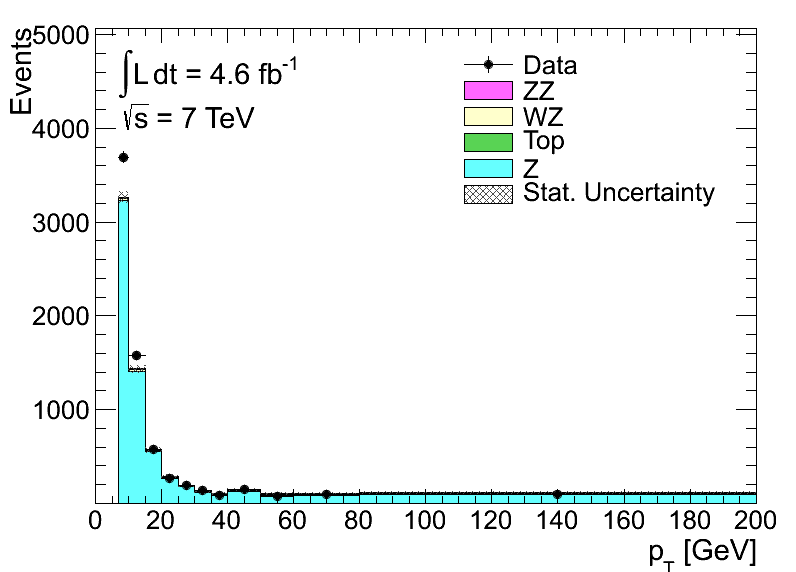
\includegraphics[width=0.47\textwidth]{ffDists/CentralEl_pt_L_lin}
%        }
%	\subfigure[Central Electron-Like-Jets]{
%            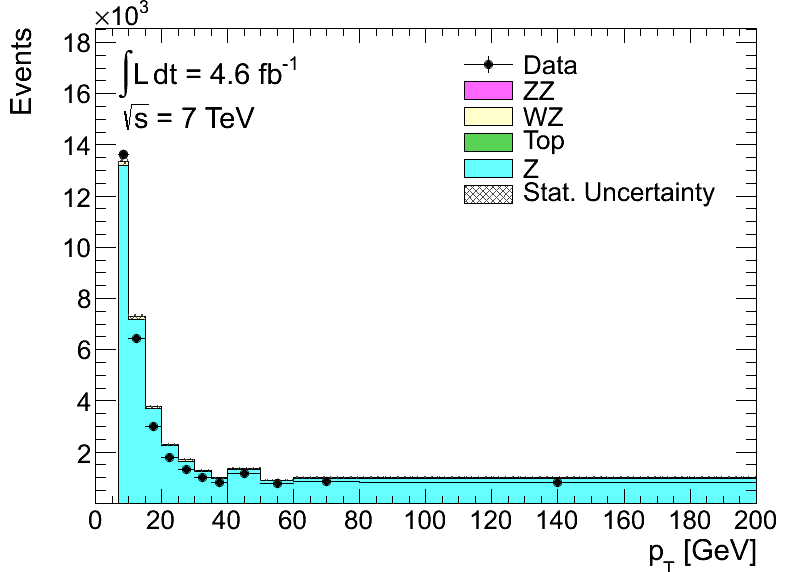
\includegraphics[width=0.47\textwidth]{ffDists/CentralEl_pt_J_lin}
%        }
%	\subfigure[Selected Forward Electrons]{
%            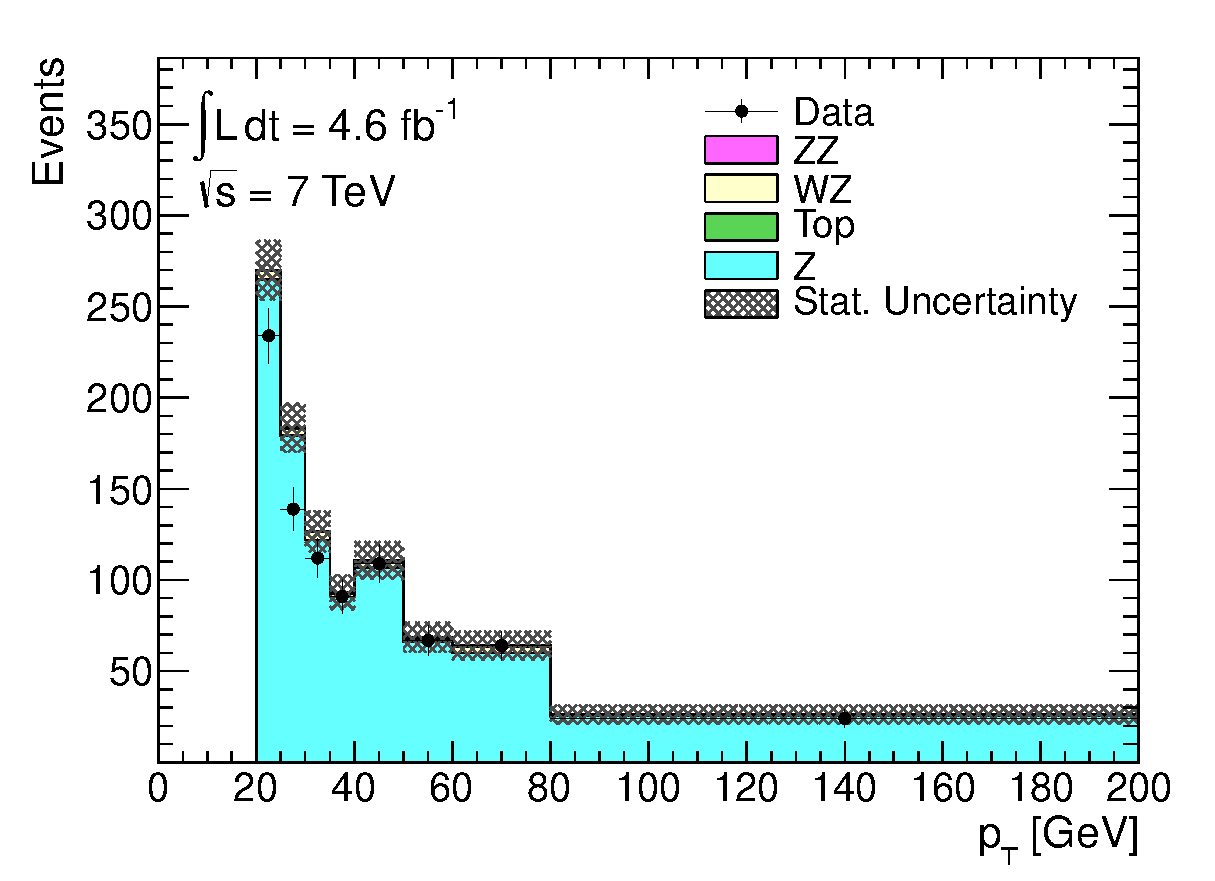
\includegraphics[width=0.47\textwidth]{ffDists/ForwardEl_pt_L_lin}
%        }
%	\subfigure[Forward Electron-Like-Jets]{
%            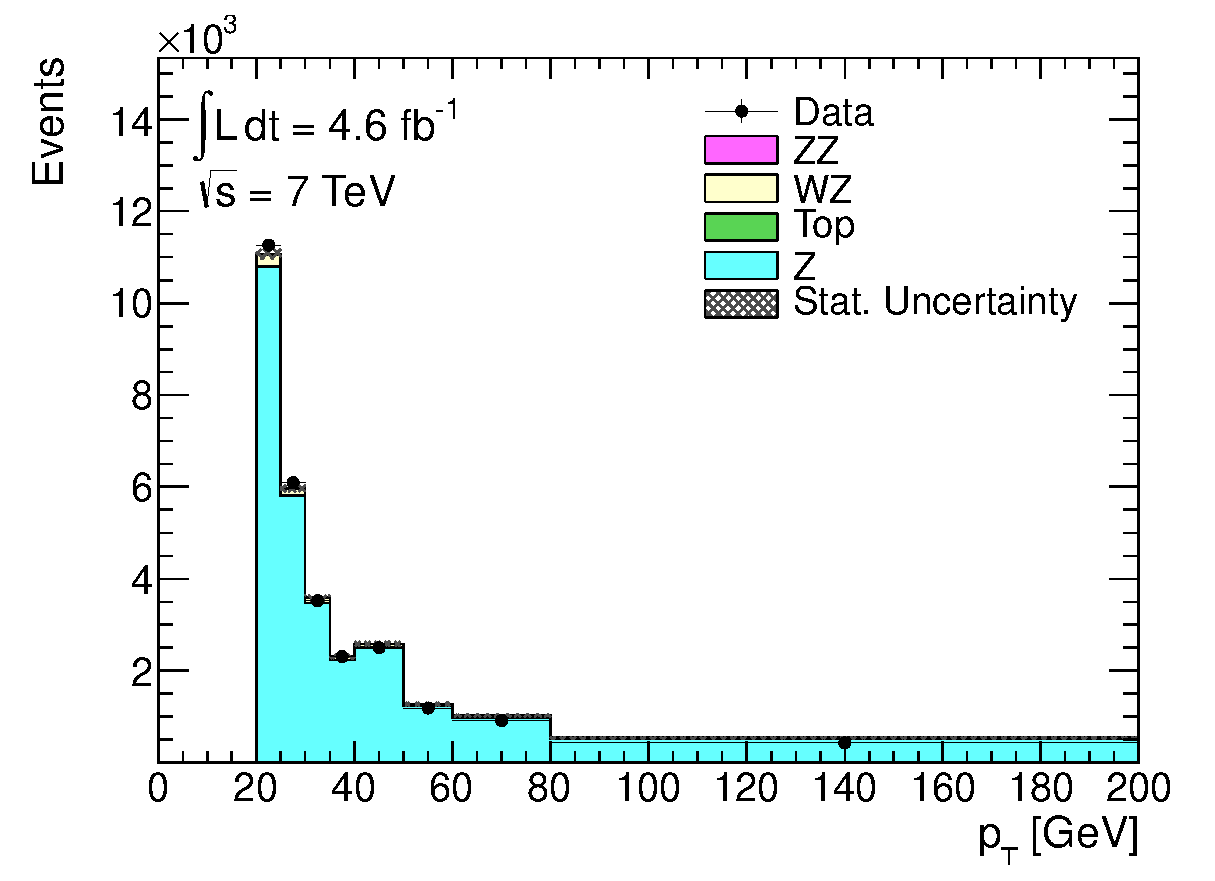
\includegraphics[width=0.47\textwidth]{ffDists/ForwardEl_pt_J_lin}
%        }
%	\subfigure[Selected Electrons]{
%            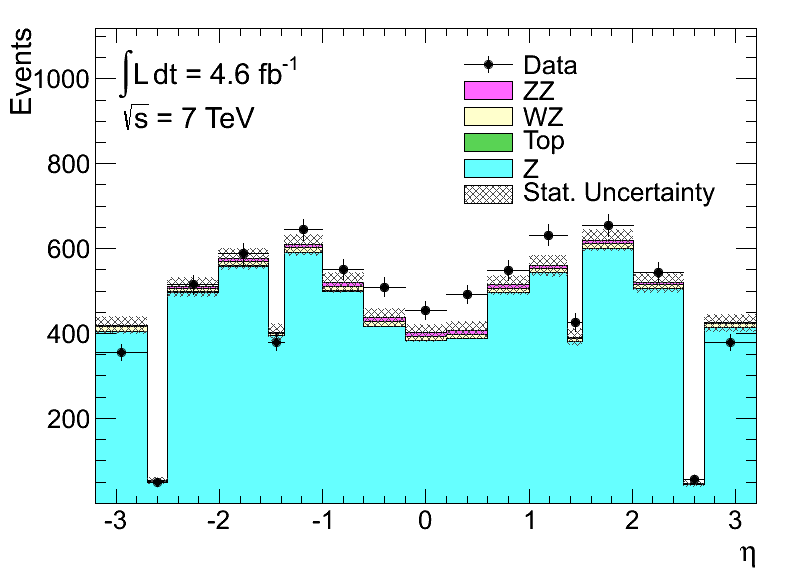
\includegraphics[width=0.47\textwidth]{ffDists/AllEl_eta_L_lin}
%        }
%	\subfigure[Electron-Like-Jets]{
%            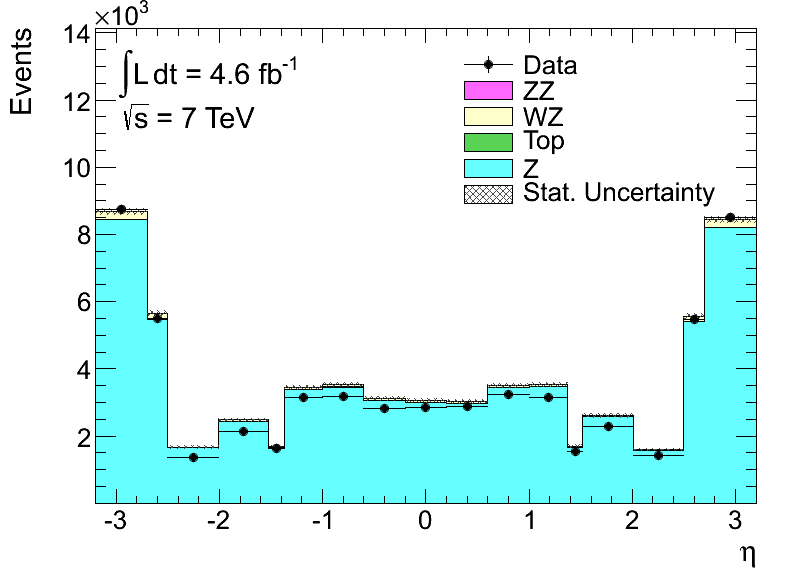
\includegraphics[width=0.47\textwidth]{ffDists/AllEl_eta_J_lin}
%        }
%    \caption[\pt\ and $\eta$ distributions for selected electrons $L$ and
%    lepton-like-electrons $J$ in the \Z-tag sample for 7~\tev\ data.]
%    {\pt\ and $\eta$ distributions for selected electrons $L$ and
%    lepton-like-electrons $J$ in the \Z-tag sample for 7~\tev\ data. 
%    For the \pt\ distributions, central and forward electrons are shown
%    separately; for the $\eta$ distributions central and forward electrons are
%    shown in the same plot.}
%\label{fig:ljdist-el-seven} 
%\end{figure}

\begin{figure}[h]
\centering
	\subfigure[Selected Central Electrons]{
            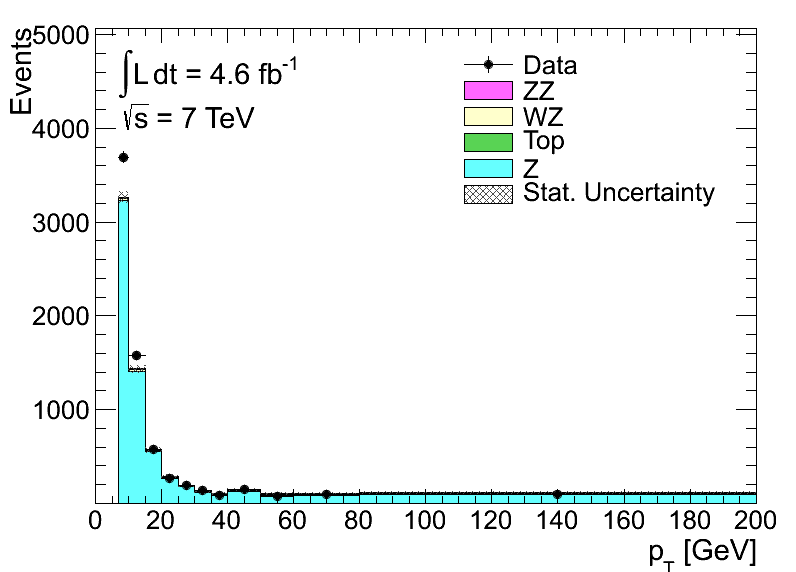
\includegraphics[width=0.47\textwidth]{ffDists/CentralEl_pt_L_lin}
        }
	\subfigure[Central Electron-Like-Jets]{
            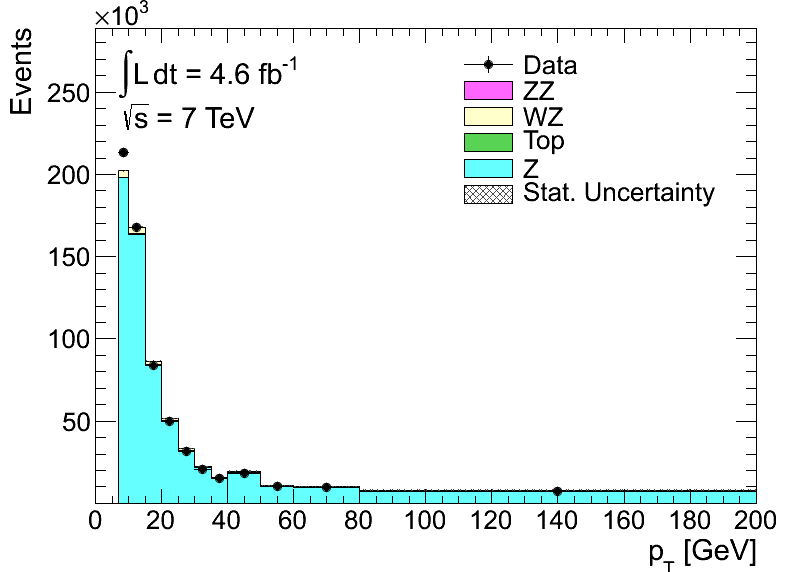
\includegraphics[width=0.47\textwidth]{ffDists/CentralEl_pt_B+C+D_lin}
        }
	\subfigure[Selected Forward Electrons]{
            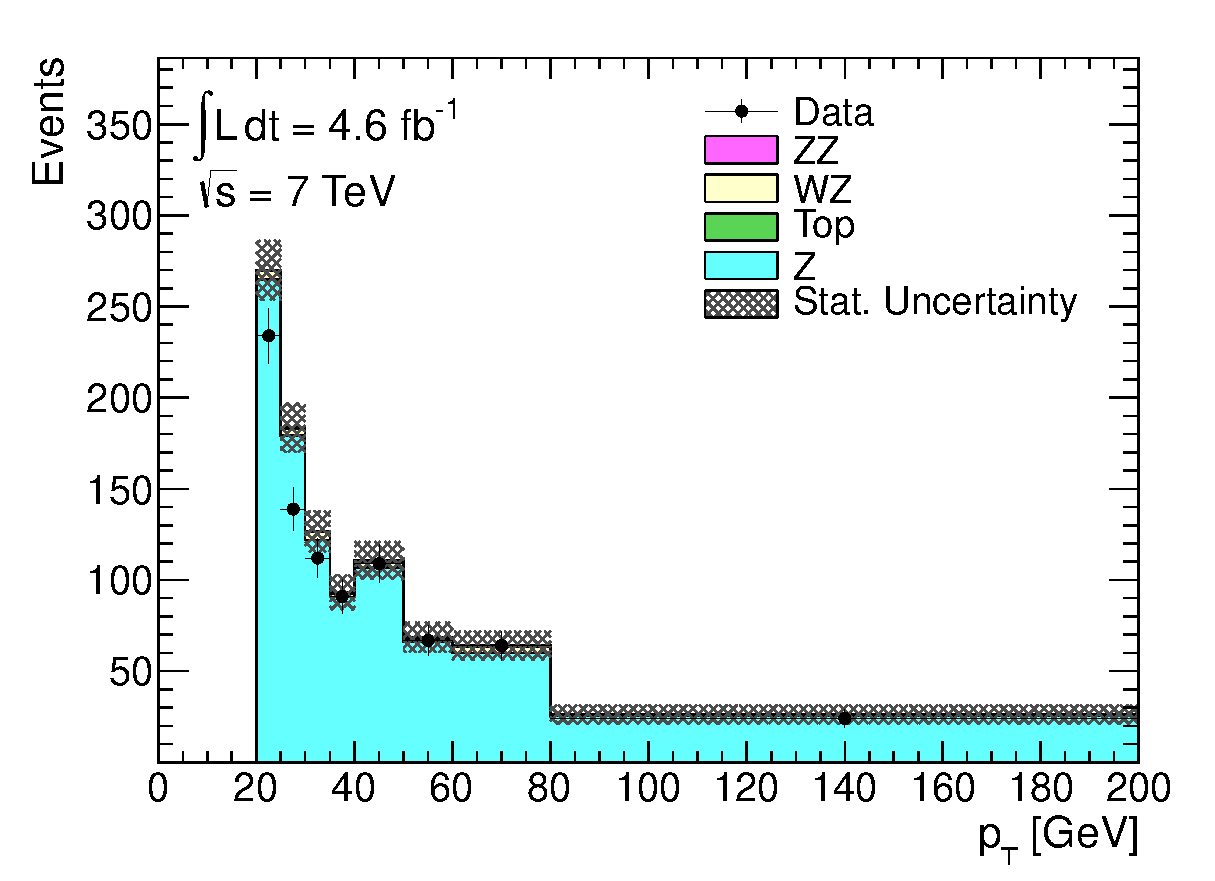
\includegraphics[width=0.47\textwidth]{ffDists/ForwardEl_pt_L_lin}
        }
	\subfigure[Forward Electron-Like-Jets]{
            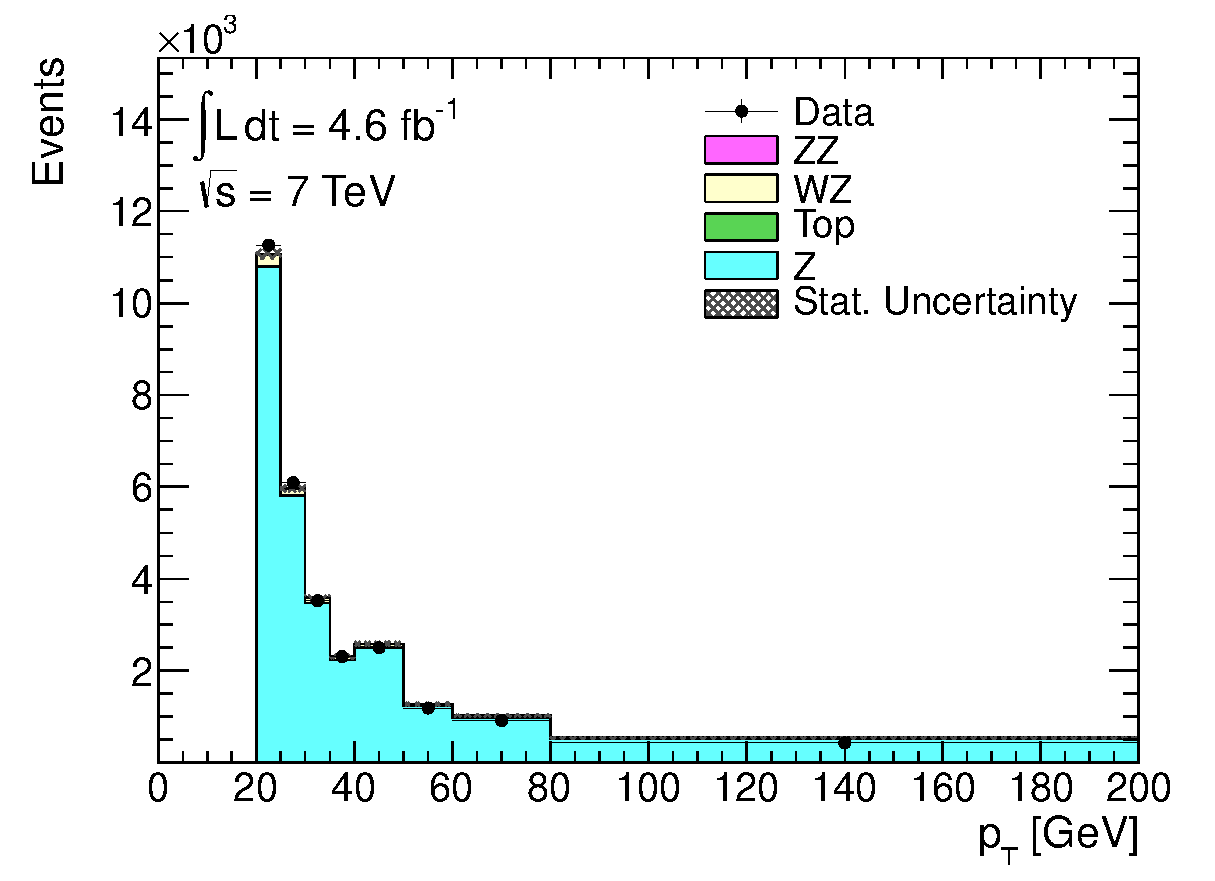
\includegraphics[width=0.47\textwidth]{ffDists/ForwardEl_pt_B+C+D_lin}
        }
	\subfigure[Selected Electrons]{
            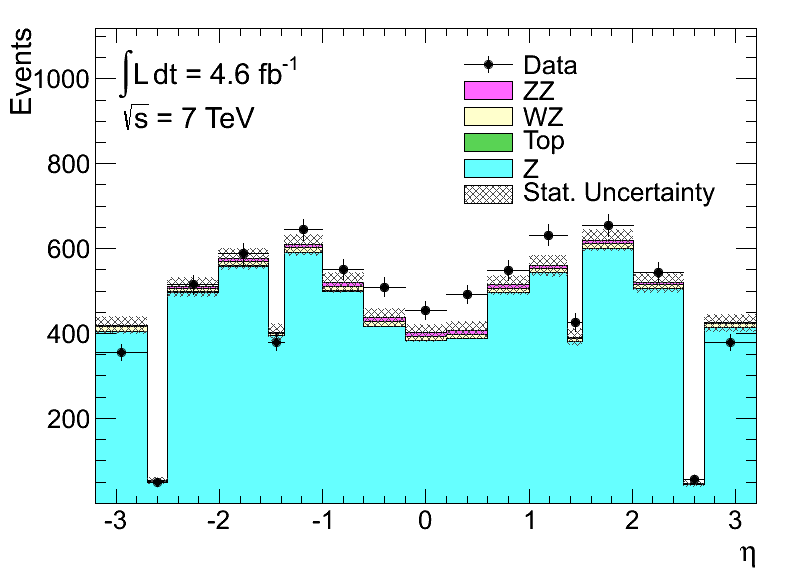
\includegraphics[width=0.47\textwidth]{ffDists/AllEl_eta_L_lin}
        }
	\subfigure[Electron-Like-Jets]{
            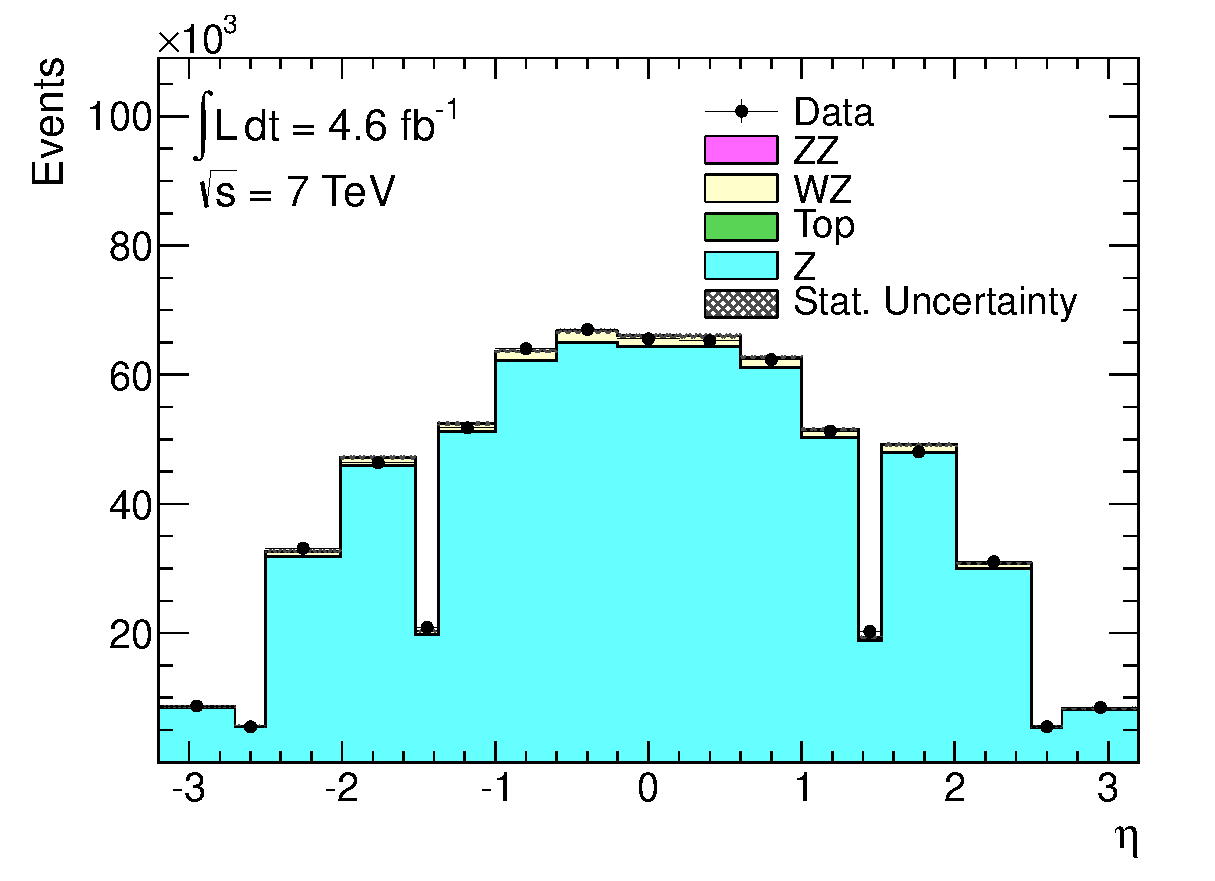
\includegraphics[width=0.47\textwidth]{ffDists/AllEl_eta_B+C+D_lin}
        }
    \caption[\pt\ and $\eta$ distributions for selected electrons $L$ and
    lepton-like-electrons $J$ in the \Z-tag sample for 7~\tev\ data.]
    {\pt\ and $\eta$ distributions for selected electrons $L$ and
    lepton-like-electrons $J$ in the \Z-tag sample for 7~\tev\ data. 
    For the \pt\ distributions, central and forward electrons are shown
    separately; for the $\eta$ distributions central and forward electrons are
    shown in the same plot.}
\label{fig:ljdist-el-seven} 
\end{figure}

%\begin{figure}[h]
%\centering
%\vspace{-8mm}
%	\subfigure[Selected Central Muons]{
%            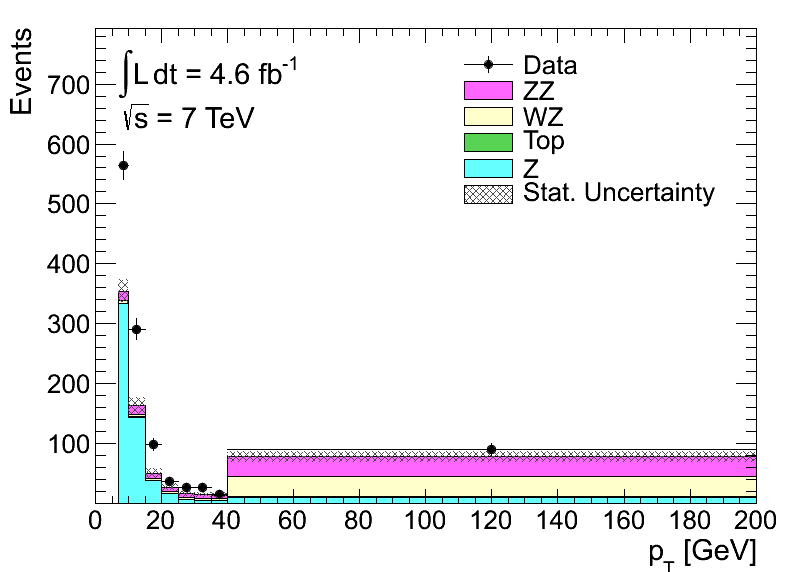
\includegraphics[width=0.47\textwidth]{ffDists/CentralMu_pt_L_lin}
%        }
%	\subfigure[Central Muon-Like-Jets]{
%            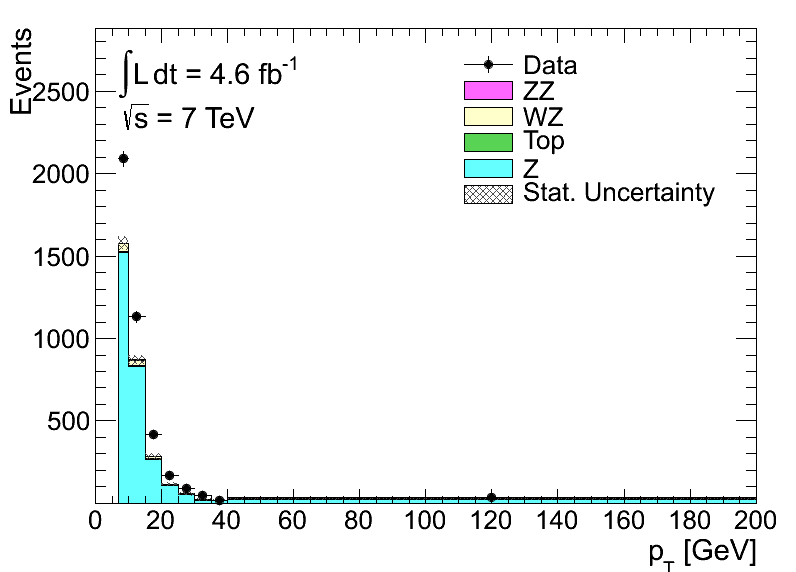
\includegraphics[width=0.47\textwidth]{ffDists/CentralMu_pt_J_lin}
%        }
%	\subfigure[Selected Forward Muons]{
%            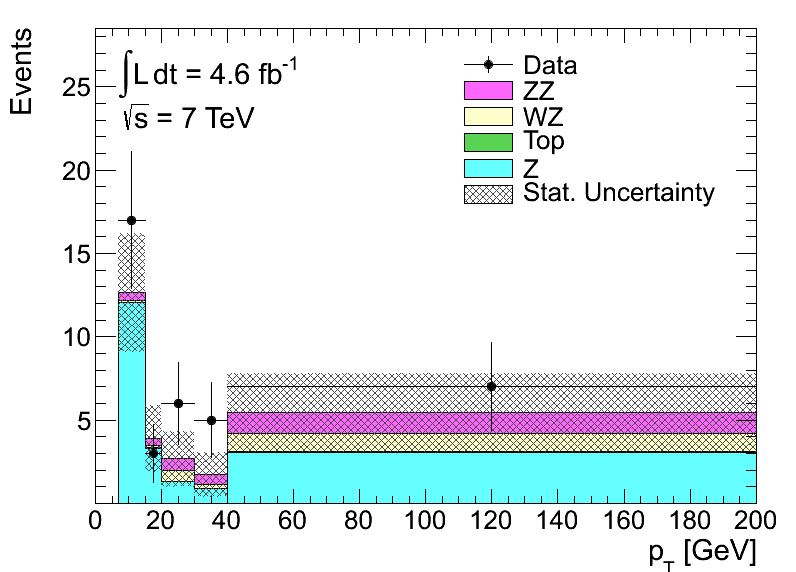
\includegraphics[width=0.47\textwidth]{ffDists/ForwardMu_pt_L_lin}
%        }
%	\subfigure[Forward Muon-Like-Jets]{
%            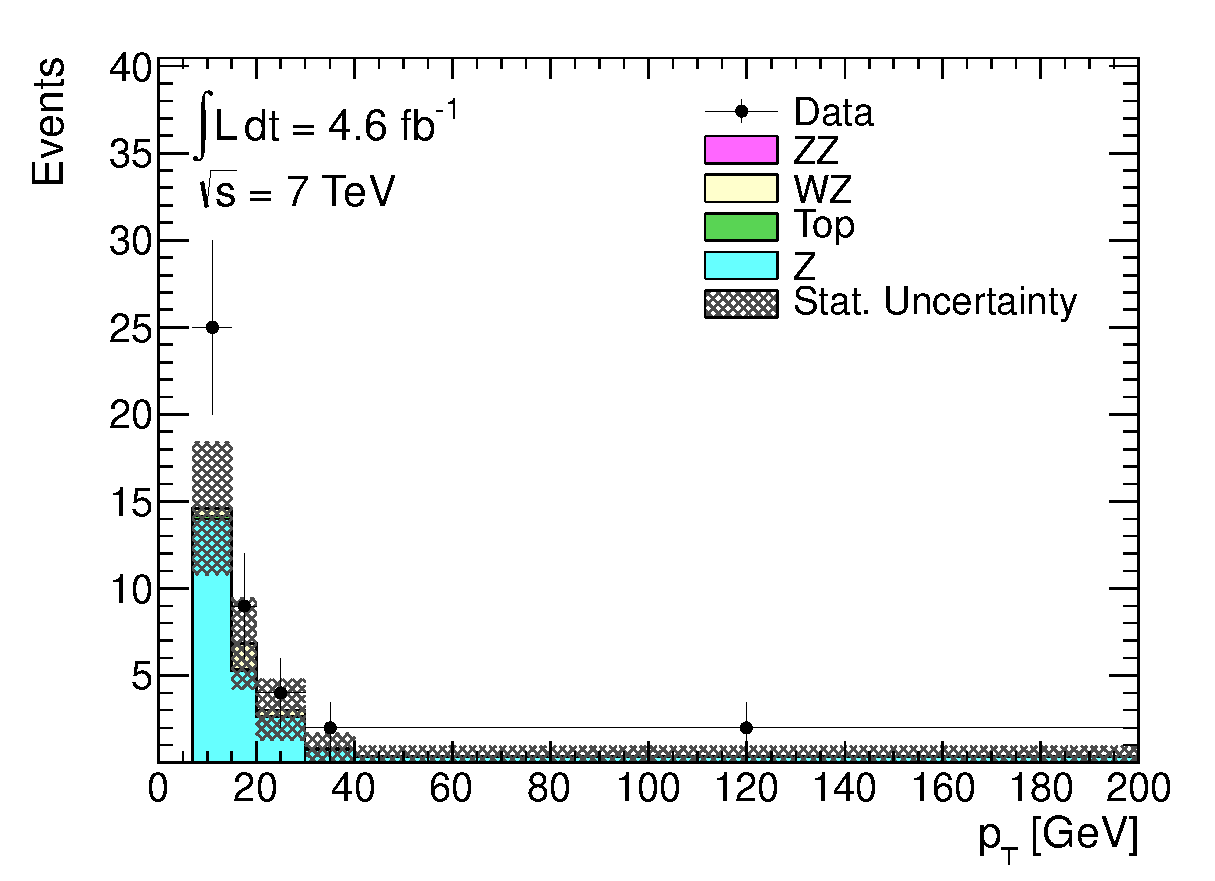
\includegraphics[width=0.47\textwidth]{ffDists/ForwardMu_pt_J_lin}
%        }
%	\subfigure[Selected Calorimeter-Tagged Muons]{
%            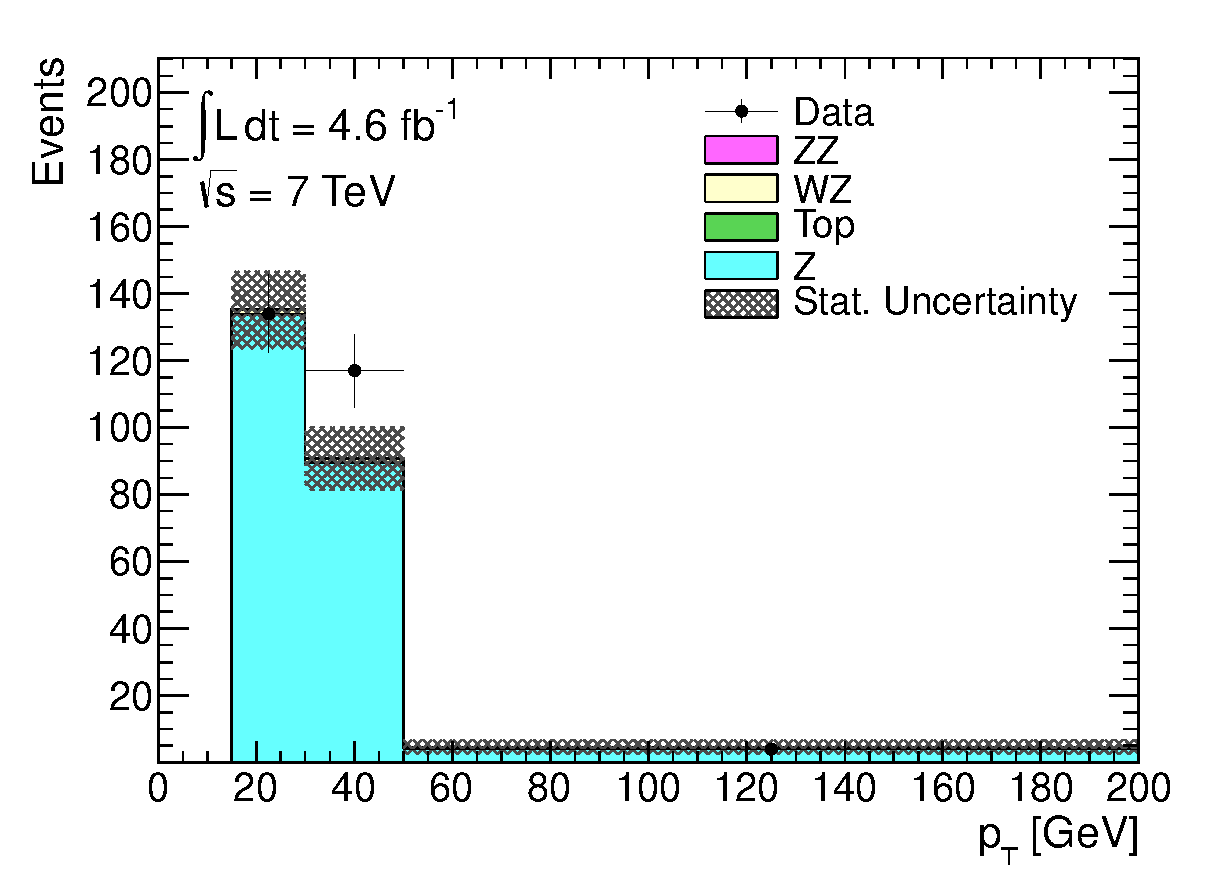
\includegraphics[width=0.47\textwidth]{ffDists/CaloMu_pt_J_lin}
%        }
%	\subfigure[Calorimeter-Tagged Muon-Like-Jets]{
%            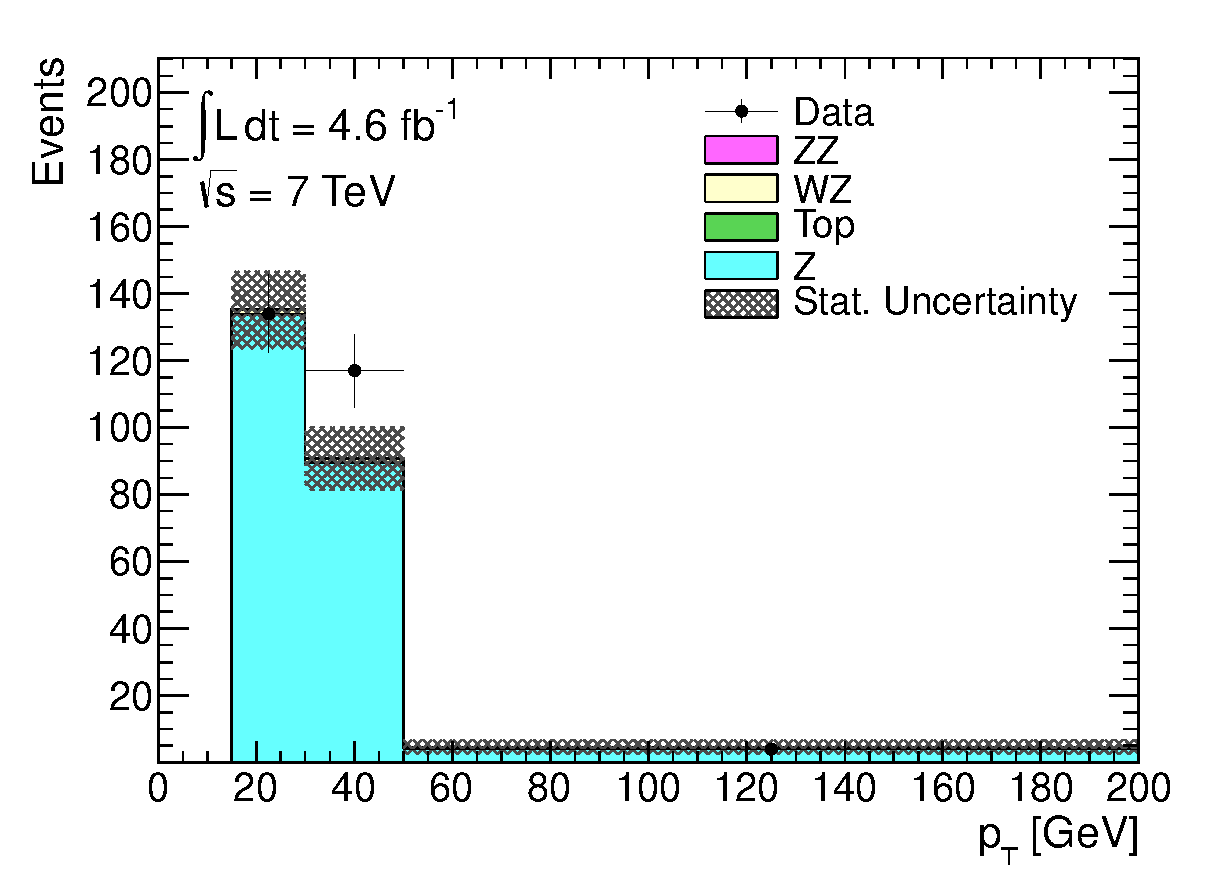
\includegraphics[width=0.47\textwidth]{ffDists/CaloMu_pt_J_lin}
%        }
%	\subfigure[Selected Muons]{
%            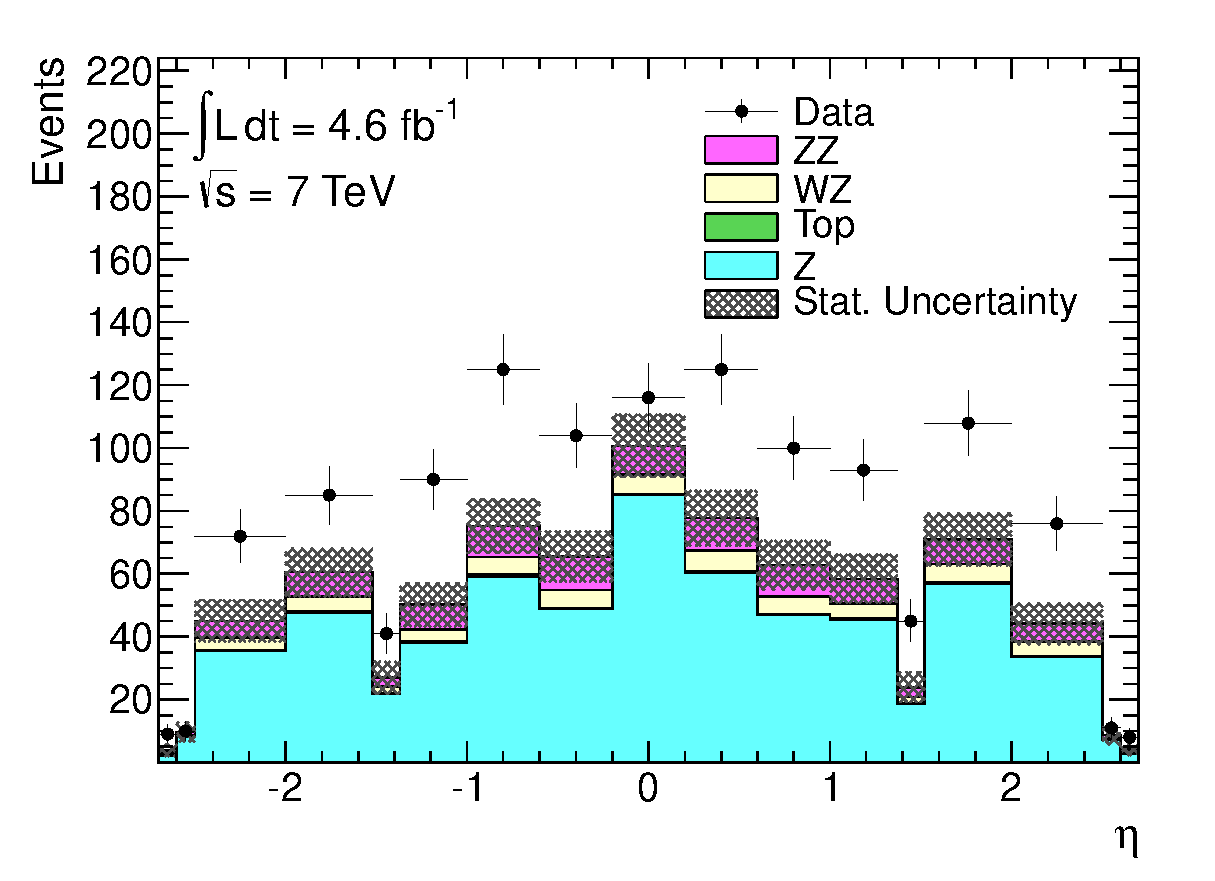
\includegraphics[width=0.47\textwidth]{ffDists/AllMu_eta_L_lin}
%        }
%	\subfigure[Muon-Like-Jets]{
%            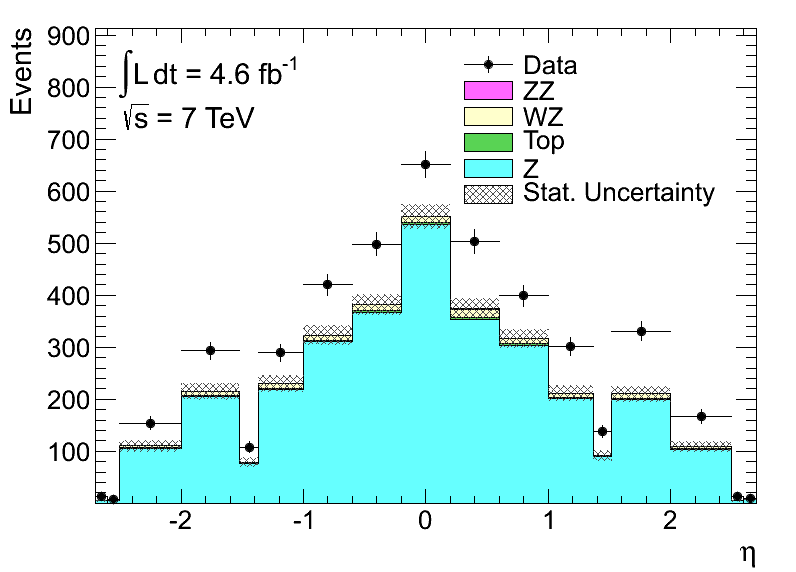
\includegraphics[width=0.47\textwidth]{ffDists/AllMu_eta_J_lin}
%        }
%    \caption[\pt\ and $\eta$ distributions for selected muons $L$ and
%    lepton-like-muons $J$ in the \Z-tag sample for 7~\tev\ data.]
%    {\small \pt\ and $\eta$ distributions for selected muons $L$ and
%    lepton-like-muons $J$ in the \Z-tag sample for 7~\tev\ data. 
%    For the \pt\ distributions, central, forward and calorimeter-tagged muons are shown
%    separately; for the $\eta$ distributions all muons are
%    shown in the same plot.}
%\label{fig:ljdist-mu-seven} 
%\end{figure}

\begin{figure}[h]
\centering
\vspace{-8mm}
	\subfigure[Selected Central Muons]{
            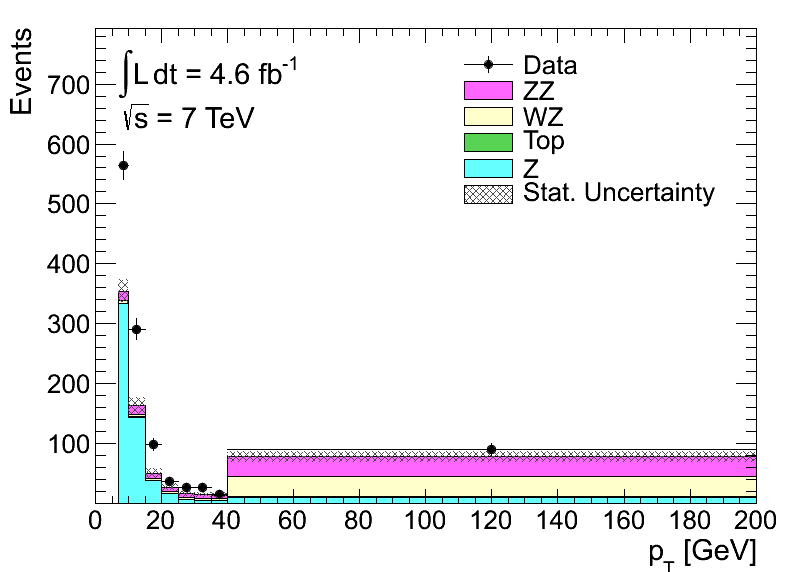
\includegraphics[width=0.47\textwidth]{ffDists/CentralMu_pt_L_lin}
        }
	\subfigure[Central Muon-Like-Jets]{
            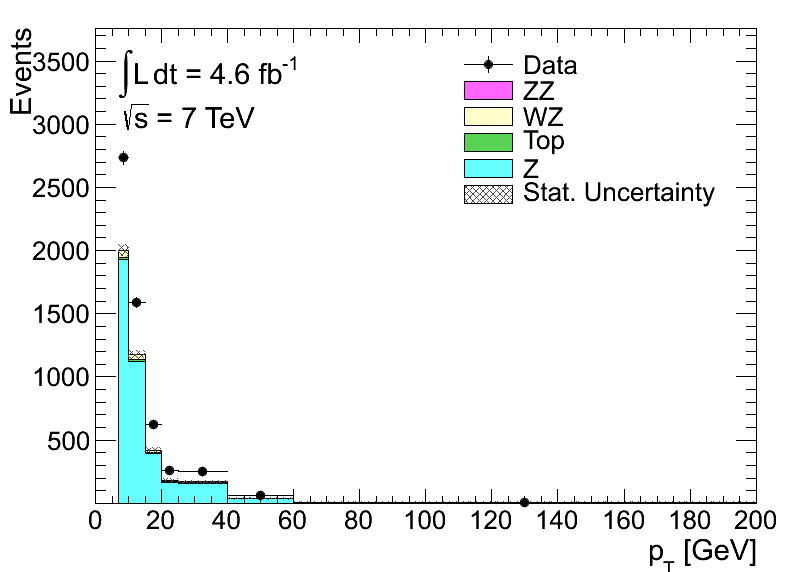
\includegraphics[width=0.47\textwidth]{ffDists/CentralMu_pt_B+C+D_lin}
        }
	\subfigure[Selected Forward Muons]{
            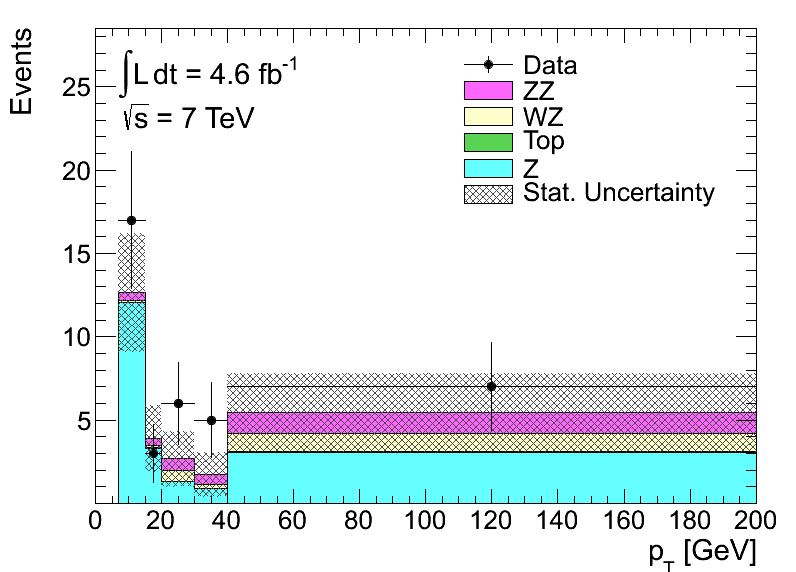
\includegraphics[width=0.47\textwidth]{ffDists/ForwardMu_pt_L_lin}
        }
	\subfigure[Forward Muon-Like-Jets]{
            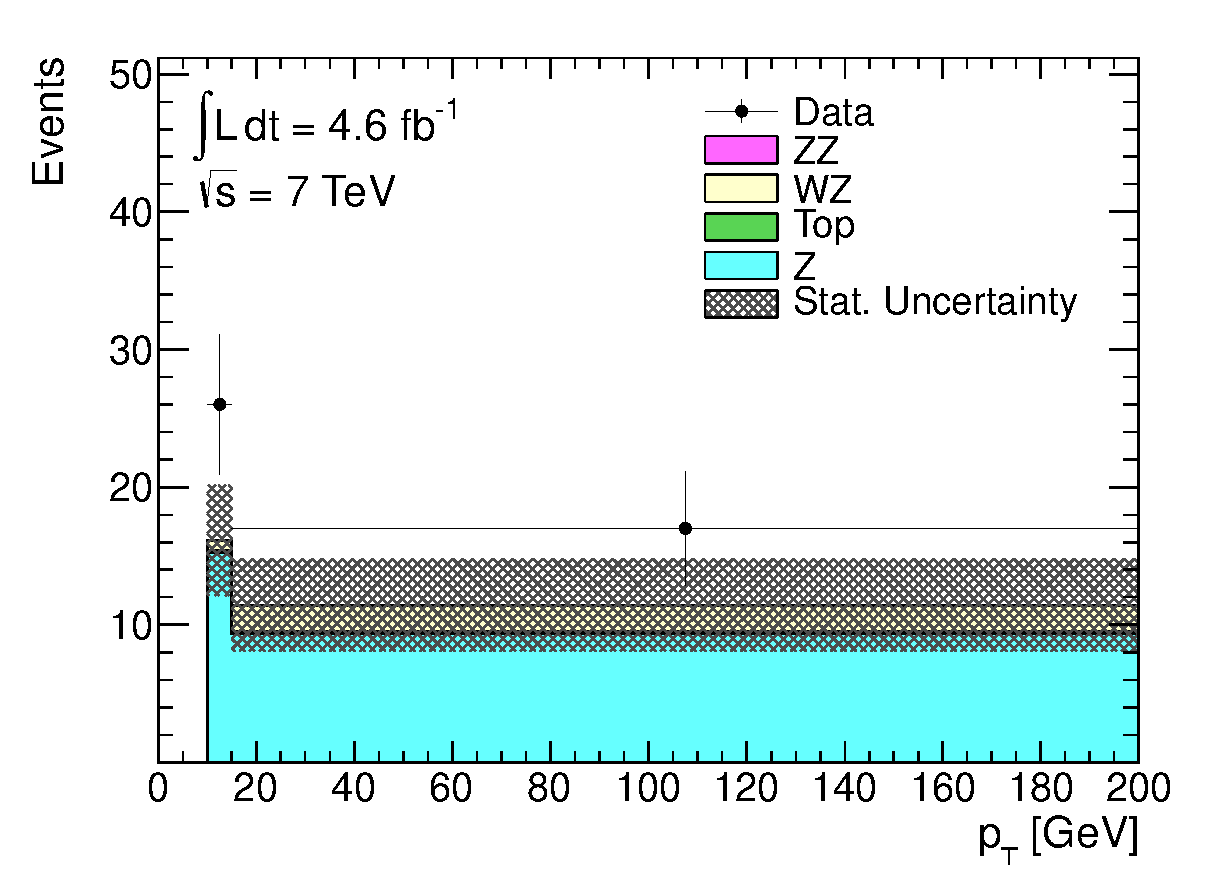
\includegraphics[width=0.47\textwidth]{ffDists/ForwardMu_pt_B+C+D_lin}
        }
	\subfigure[Selected Calorimeter-Tagged Muons]{
            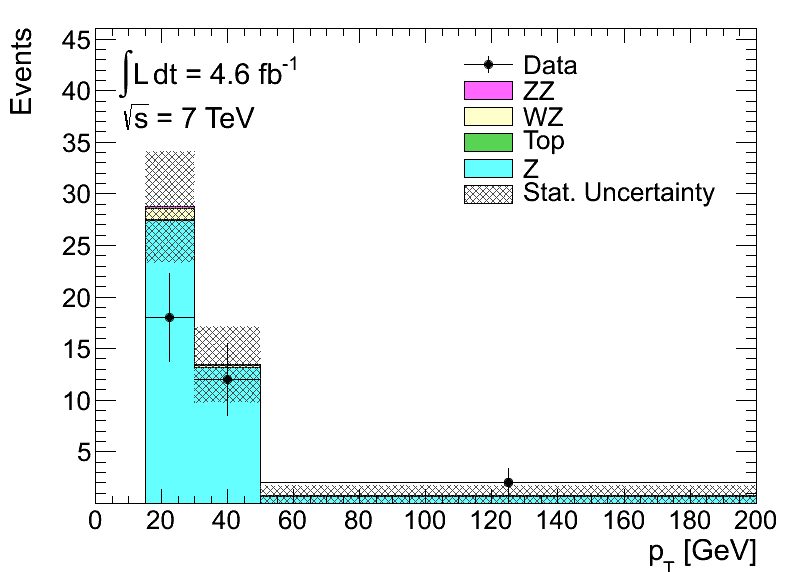
\includegraphics[width=0.47\textwidth]{ffDists/CaloMu_pt_L_lin}
        }
	\subfigure[Calorimeter-Tagged Muon-Like-Jets]{
            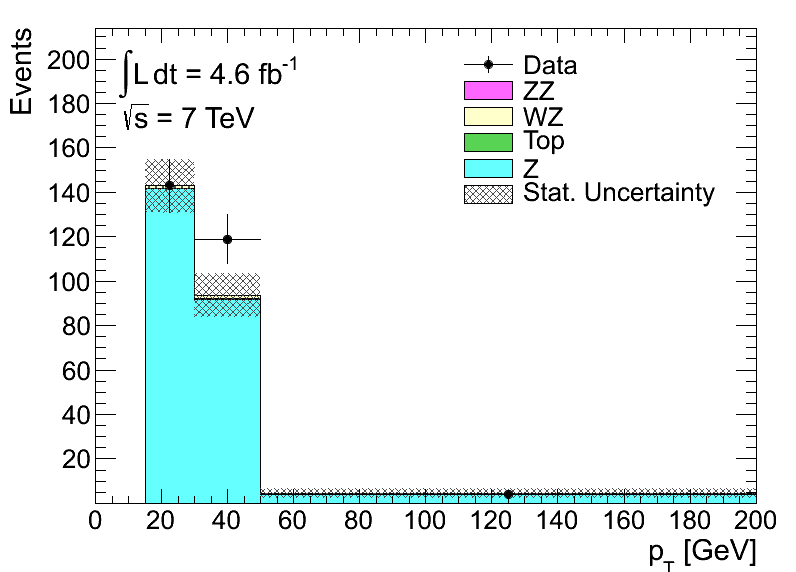
\includegraphics[width=0.47\textwidth]{ffDists/CaloMu_pt_B+C+D_lin}
        }
	\subfigure[Selected Muons]{
            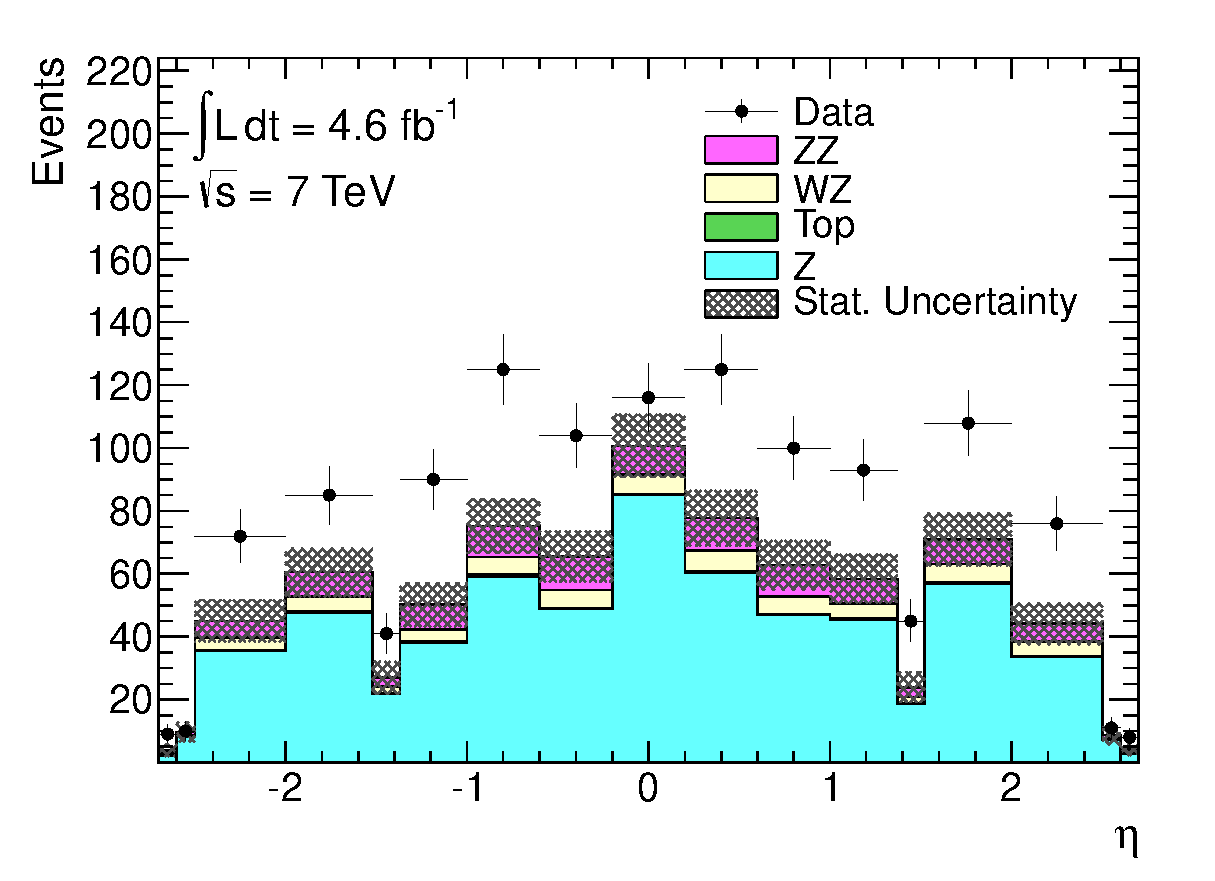
\includegraphics[width=0.47\textwidth]{ffDists/AllMu_eta_L_lin}
        }
	\subfigure[Muon-Like-Jets]{
            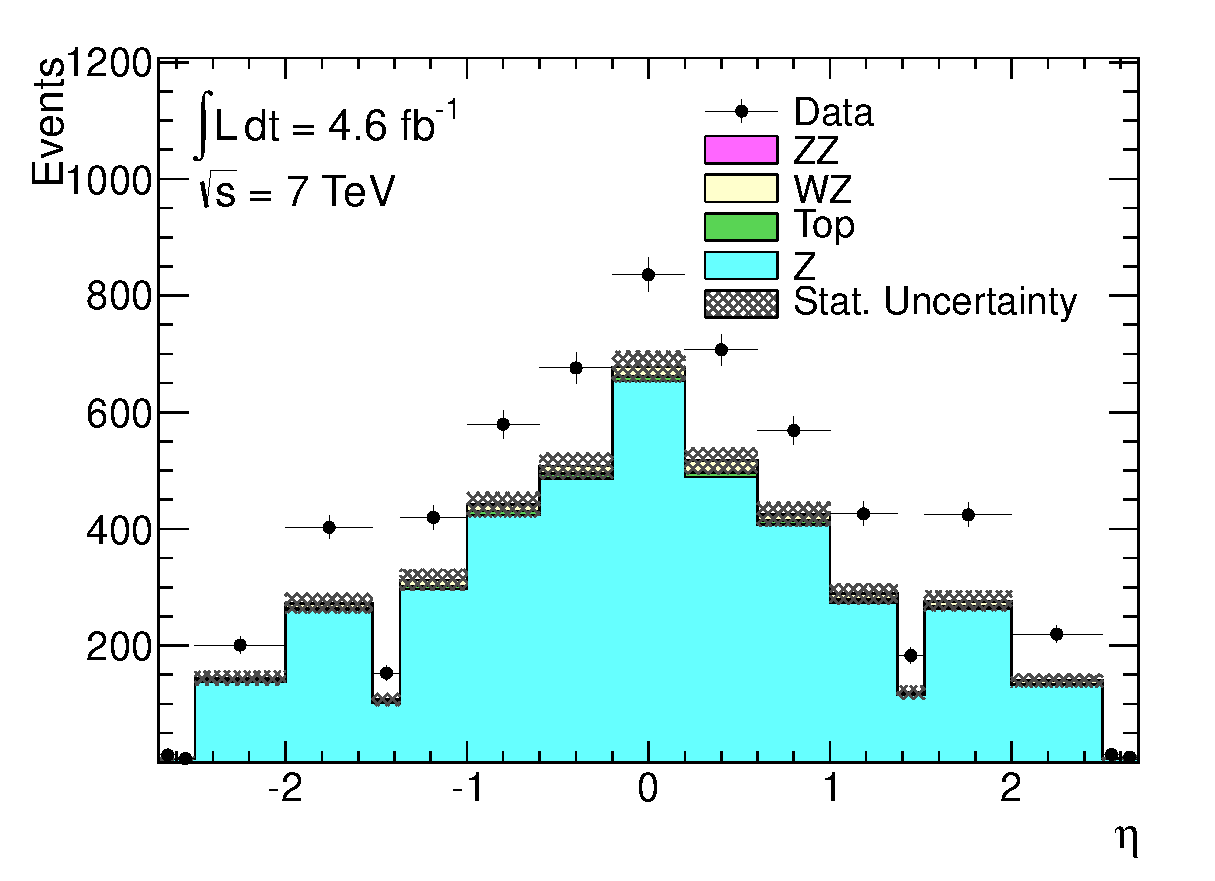
\includegraphics[width=0.47\textwidth]{ffDists/AllMu_eta_B+C+D_lin}
        }
    \caption[\pt\ and $\eta$ distributions for selected muons $L$ and
    lepton-like-muons $J$ in the \Z-tag sample for 7~\tev\ data.]
    {\small \pt\ and $\eta$ distributions for selected muons $L$ and
    lepton-like-muons $J$ in the \Z-tag sample for 7~\tev\ data. 
    For the \pt\ distributions, central, forward and calorimeter-tagged muons are shown
    separately; for the $\eta$ distributions all muons are
    shown in the same plot.}
\label{fig:ljdist-mu-seven} 
\end{figure}

The observed \fakefactor s for electrons are shown in~\fig{ff-el-seven} for the
7~\tev\ analysis and in~\fig{ff-el-eight} for the 8~\tev\ analysis; the \fakefactor s
for muons are shown in~\fig{ff-mu-seven} for the
7~\tev\ analysis and in~\fig{ff-mu-eight} for the 8~\tev\ analysis. The
\ffactor\ estimated from \mc\ (blue triangles) is in reasonable agreement with
the \ffactor\ measured in data (black points). For the calculation of the
background, no use is made of the \ffactor\ estimated from \mc. The average \FF
s, used as the numerator in~\eqn{factorised-ff}, are given in~\tab{average-ff}.

\begin{table}[htbp]
  \centering
  \small
  \begin{tabular}{lcc} 
    \hline\hline
    Lepton & $<\FF>$ 7~\tev &  $<\FF>$ 8~\tev \\
    \hline
    Central Electron            & \measStat{0.215}{\errSym{0.003}} & \\
    Forward Electron            & \measStat{0.030}{\errSym{0.001}} & \\
    Central Muon                & \measStat{0.250}{\errSym{0.010}} & \\
    Forward Muon                & \measStat{0.782}{\errSym{0.199}} & \\
    Calorimeter-Tagged Muon     & \measStat{0.123}{\errSym{0.024}} &  \\
    \hline\hline
  \end{tabular}
  \caption{Average \ffactor s for different lepton types.}
  \label{table:average-ff}
\end{table}

\begin{figure}[h]
\centering
	\subfigure[Central Electrons]{
            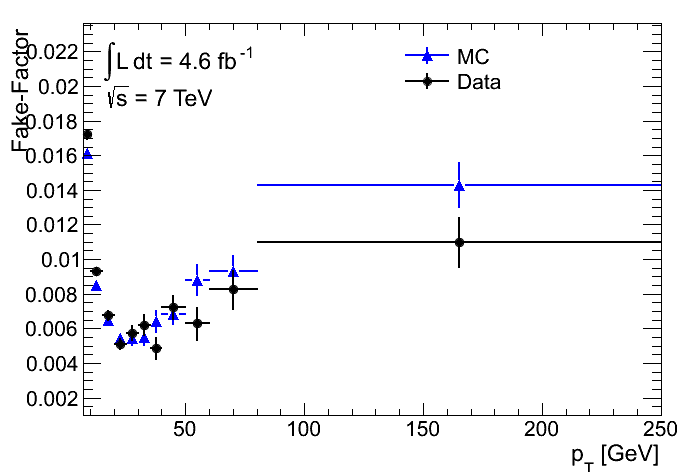
\includegraphics[width=0.47\textwidth]{FakeFactors/FF_CentralEl_pt_B+C+D_lin}
        }
	\subfigure[Forward Electrons]{
            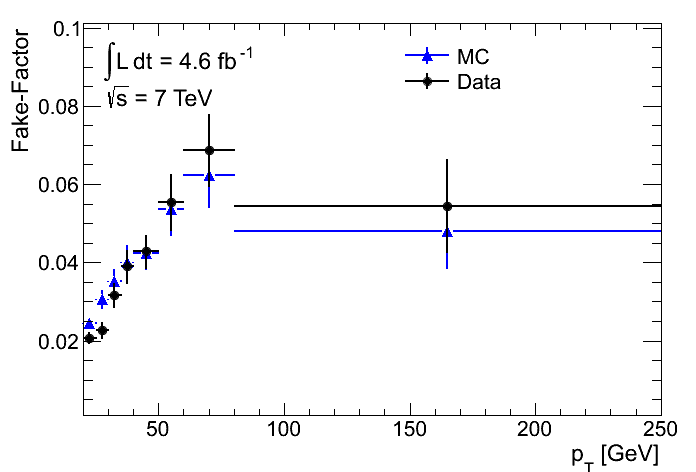
\includegraphics[width=0.47\textwidth]{FakeFactors/FF_ForwardEl_pt_B+C+D_lin}
        }
	\subfigure[All Electrons]{
            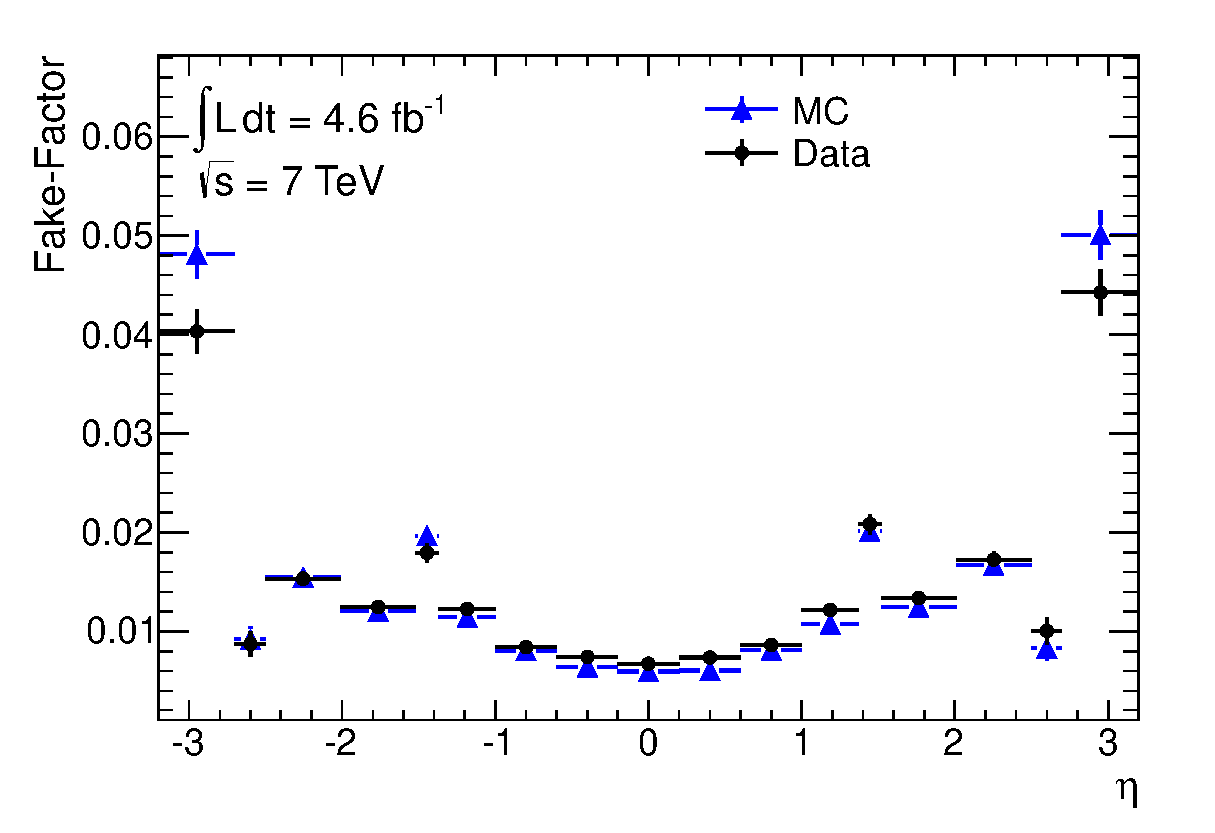
\includegraphics[width=0.47\textwidth]{FakeFactors/FF_AllEl_eta_B+C+D_lin}
        }
    \caption[Electron \FakeFactor s as a function of \pt\ and $\eta$ for 7~\tev\ data.]
    {Electron \FakeFactor s as a function of \pt\ and $\eta$ for 7~\tev\ data. 
    For the distributions as a function of \pt\, central and forward electrons are shown
    separately; for the $\eta$ distributions the \ffactor\ for central and forward electrons are
    shown in the same plot. The black points show the \ffactor\ measured in
    data; the blue triangles show the value estimated by \mc.}
\label{fig:ff-el-seven} 
\end{figure}

%\begin{figure}[h]
%\centering
%	\subfigure[Central Electrons]{
%            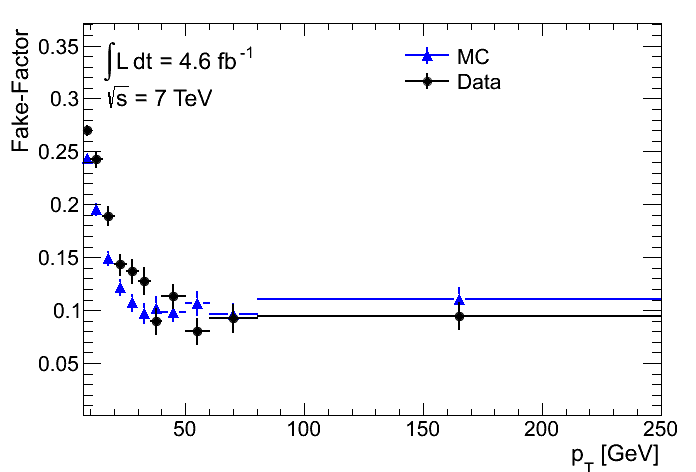
\includegraphics[width=0.47\textwidth]{FakeFactors/FF_CentralEl_pt_J_lin}
%        }
%	\subfigure[Forward Electrons]{
%            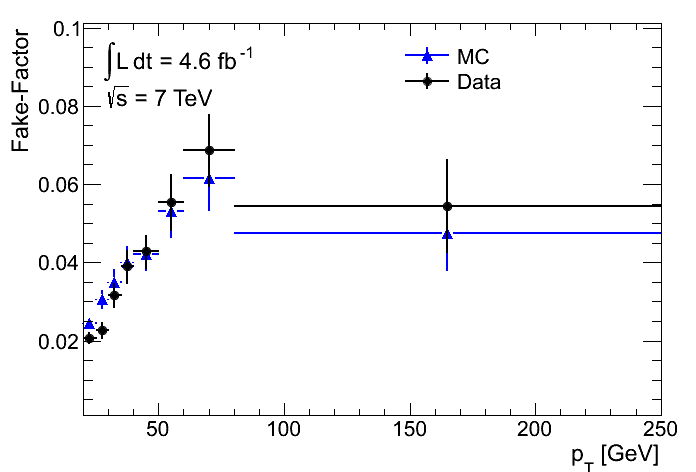
\includegraphics[width=0.47\textwidth]{FakeFactors/FF_ForwardEl_pt_J_lin}
%        }
%	\subfigure[All Electrons]{
%            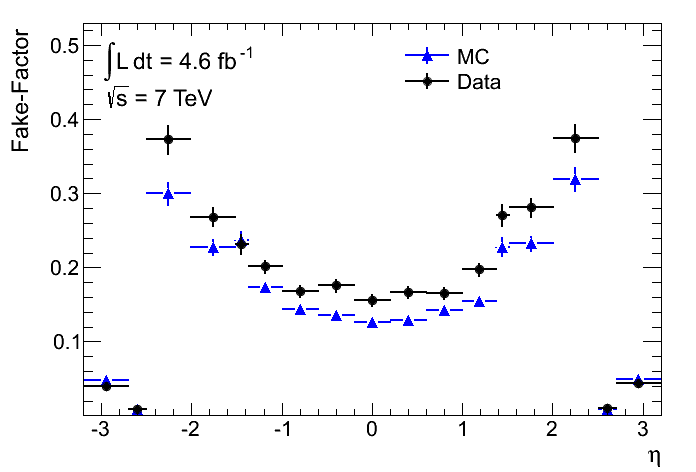
\includegraphics[width=0.47\textwidth]{FakeFactors/FF_AllEl_eta_J_lin}
%        }
%    \caption[Electron \FakeFactor s as a function of \pt\ and $\eta$ for 7~\tev\ data.]
%    {Electron \FakeFactor s as a function of \pt\ and $\eta$ for 7~\tev\ data. 
%    For the distributions as a function of \pt\, central and forward electrons are shown
%    separately; for the $\eta$ distributions the \ffactor\ for central and forward electrons are
%    shown in the same plot. The black points show the \ffactor\ measured in
%    data; the blue triangles show the value estimated by \mc.}
%\label{fig:ff-el-seven} 
%\end{figure}
%
%\begin{figure}[h]
%\centering
%	\subfigure[Central Electrons]{
%            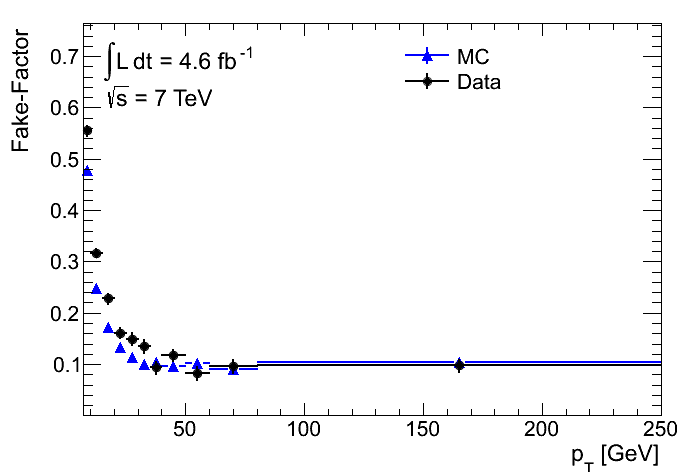
\includegraphics[width=0.47\textwidth]{FakeFactors/FF_CentralEl_pt_B_lin}
%        }
%	\subfigure[Forward Electrons]{
%            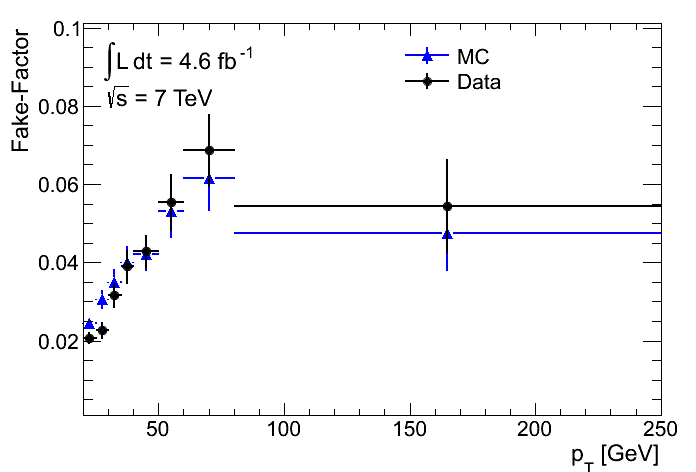
\includegraphics[width=0.47\textwidth]{FakeFactors/FF_ForwardEl_pt_B_lin}
%        }
%	\subfigure[All Electrons]{
%            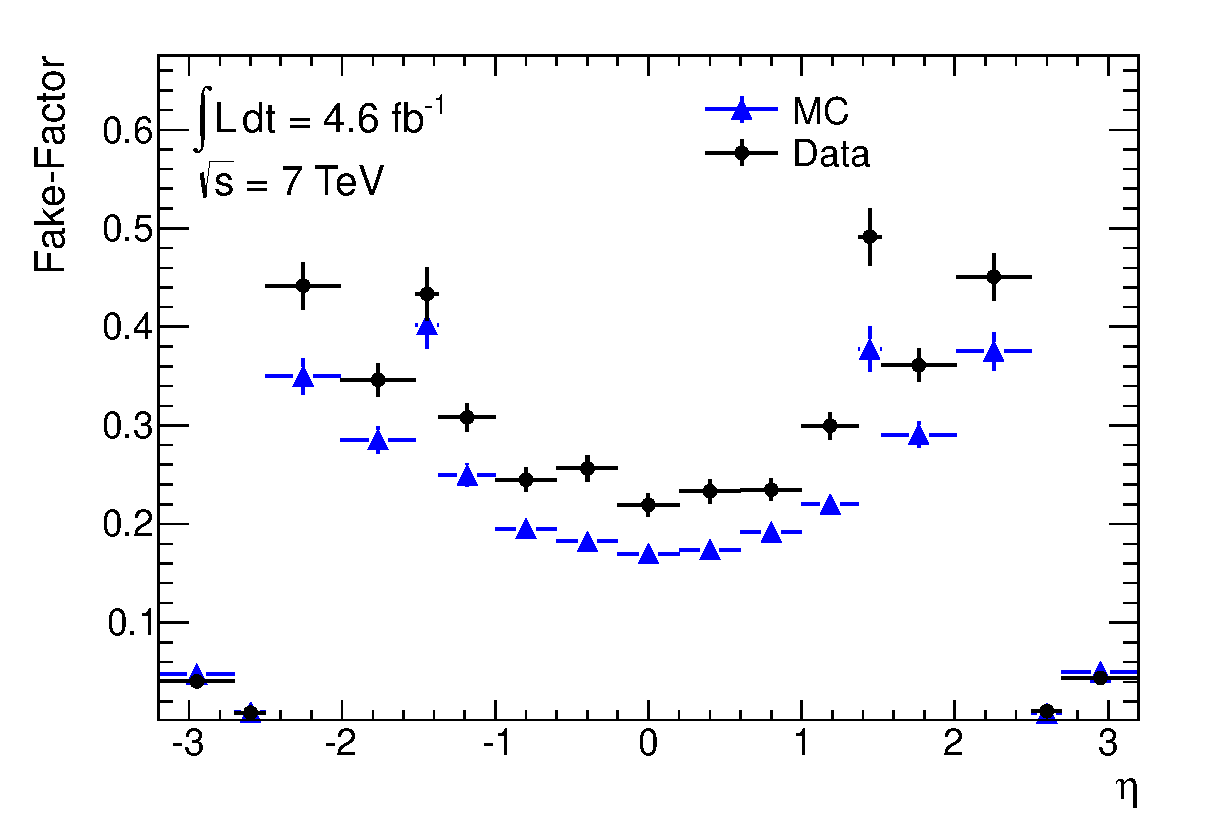
\includegraphics[width=0.47\textwidth]{FakeFactors/FF_AllEl_eta_B_lin}
%        }
%    \caption[Electron \FakeFactor s as a function of \pt\ and $\eta$ for 7~\tev\ data.]
%    {Electron \FakeFactor s as a function of \pt\ and $\eta$ for 7~\tev\ data. 
%    For the distributions as a function of \pt\, central and forward electrons are shown
%    separately; for the $\eta$ distributions the \ffactor\ for central and forward electrons are
%    shown in the same plot. The black points show the \ffactor\ measured in
%    data; the blue triangles show the value estimated by \mc.}
%\label{fig:ff-el-seven} 
%\end{figure}

\begin{figure}[h]
\centering
\vspace{-8mm}
	\subfigure[Central Muons]{
            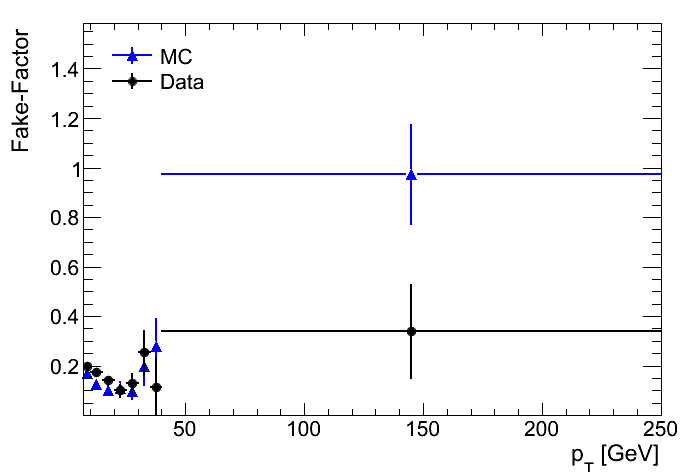
\includegraphics[width=0.47\textwidth]{FakeFactors/FF_CentralMu_pt_B+C+D_lin}
        }
	\subfigure[Forward Muons]{
            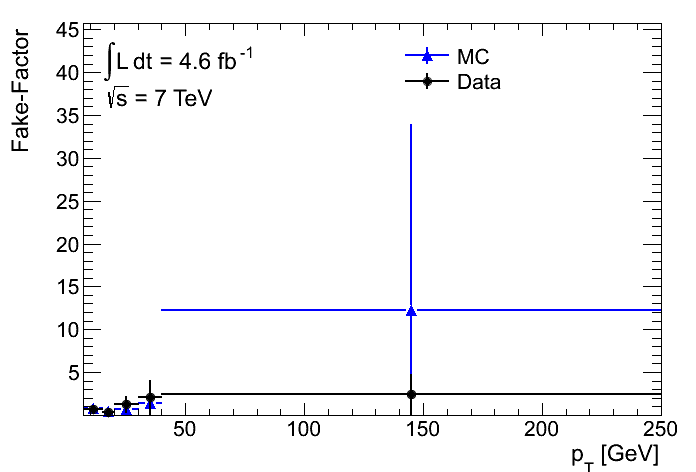
\includegraphics[width=0.47\textwidth]{FakeFactors/FF_ForwardMu_pt_B+C+D_lin}
        }
	\subfigure[Calorimeter-Tagged Muons]{
            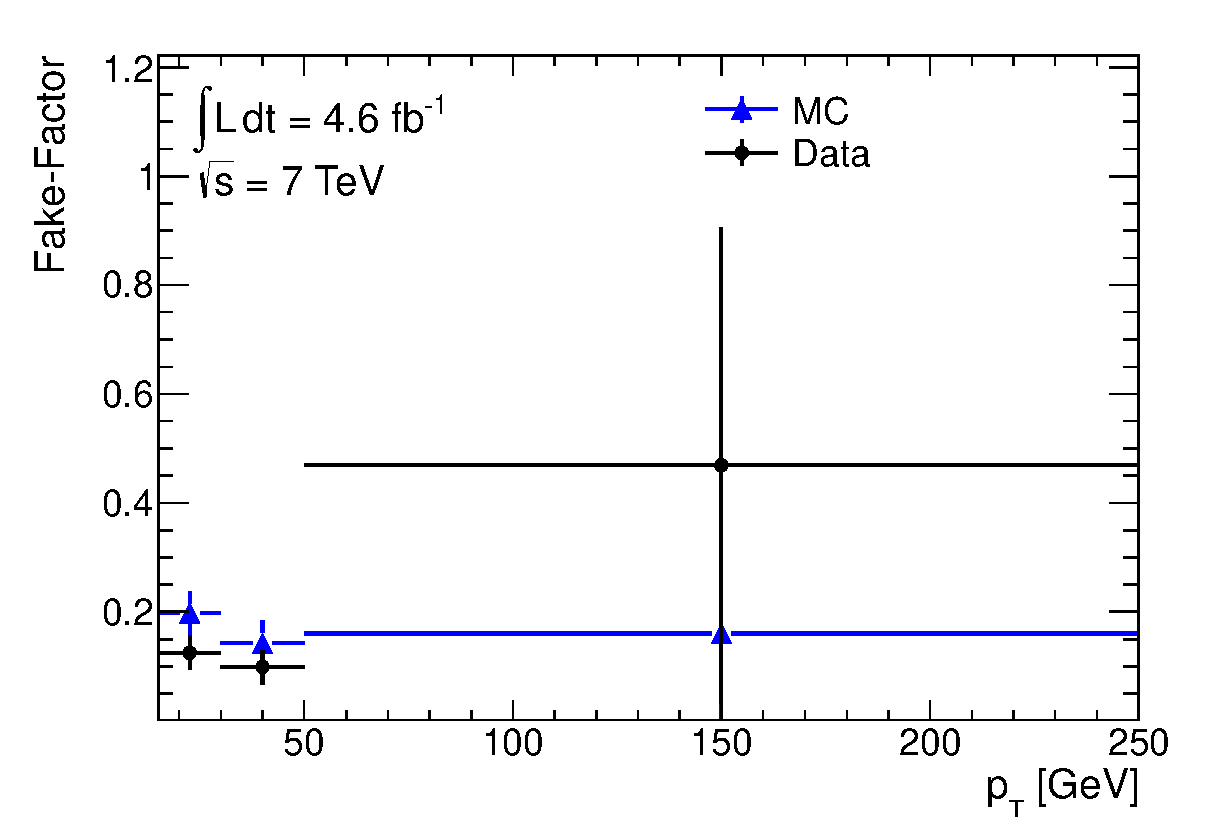
\includegraphics[width=0.47\textwidth]{FakeFactors/FF_CaloMu_pt_B+C+D_lin}
        }
	\subfigure[All Muons]{
            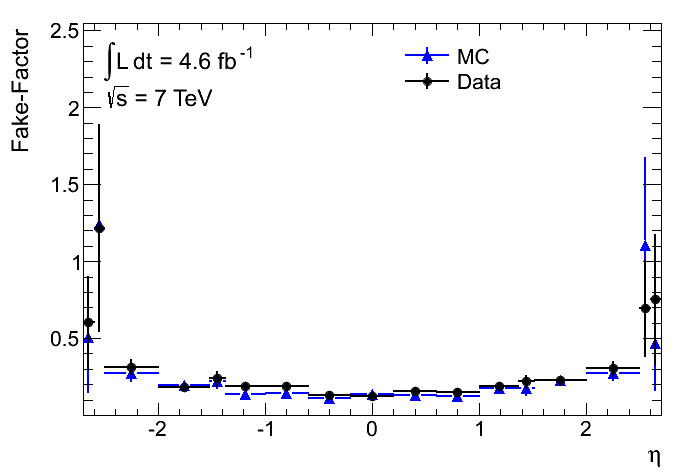
\includegraphics[width=0.47\textwidth]{FakeFactors/FF_AllMu_eta_B+C+D_lin}
        }
    \caption[Muon \FakeFactor s as a function of \pt\ and $\eta$ for 7~\tev\ data.]
    {Muon \FakeFactor s as a function of \pt\ and $\eta$ for 7~\tev\ data. 
    For the distributions as a function of \pt\, central, forward and calorimeter-tagged muons are shown
    separately; for the $\eta$ distributions the \ffactor\ all electrons are
    shown in the same plot.The black points show the \ffactor\ measured in
    data; the blue triangles show the value estimated by \mc.}
\label{fig:ff-mu-seven} 
\end{figure}

%\begin{figure}[h]
%\centering
%\vspace{-8mm}
%	\subfigure[Central Muons]{
%            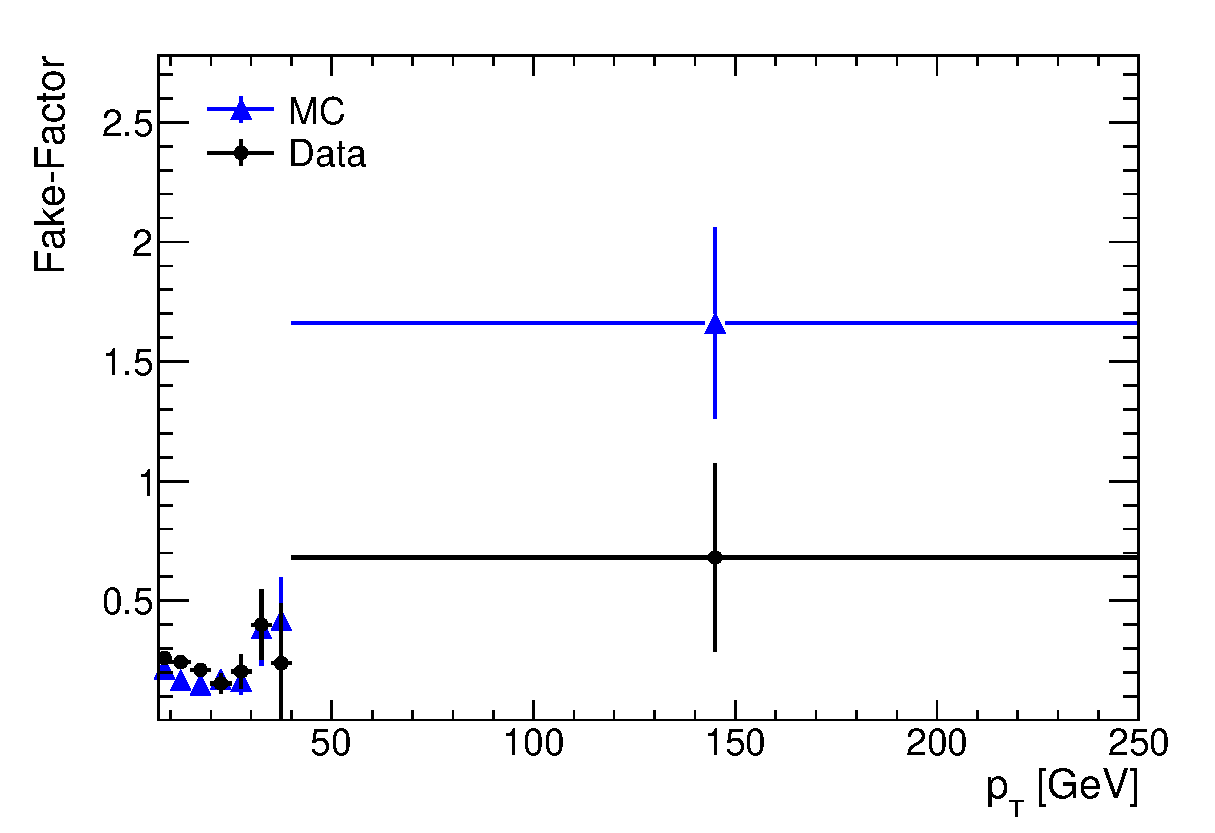
\includegraphics[width=0.47\textwidth]{FakeFactors/FF_CentralMu_pt_J_lin}
%        }
%	\subfigure[Forward Muons]{
%            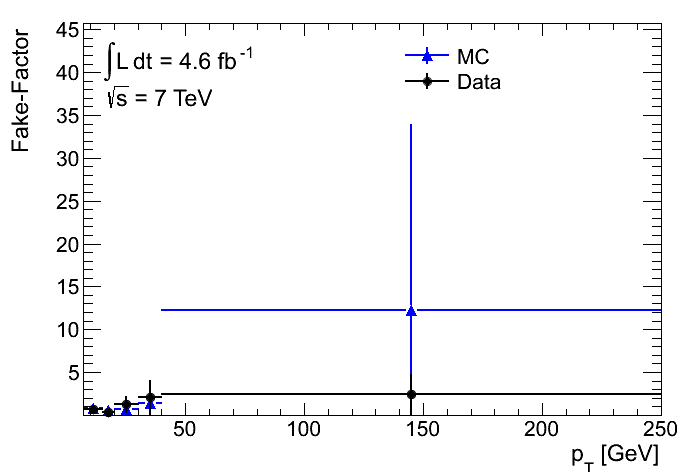
\includegraphics[width=0.47\textwidth]{FakeFactors/FF_ForwardMu_pt_J_lin}
%        }
%	\subfigure[Calorimeter-Tagged Muons]{
%            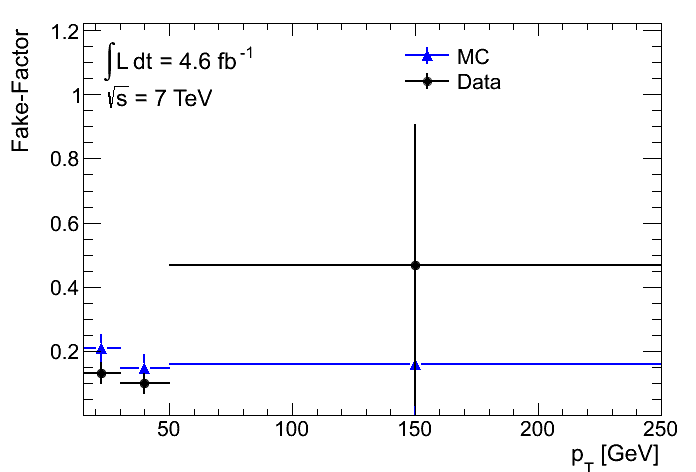
\includegraphics[width=0.47\textwidth]{FakeFactors/FF_CaloMu_pt_J_lin}
%        }
%	\subfigure[All Muons]{
%            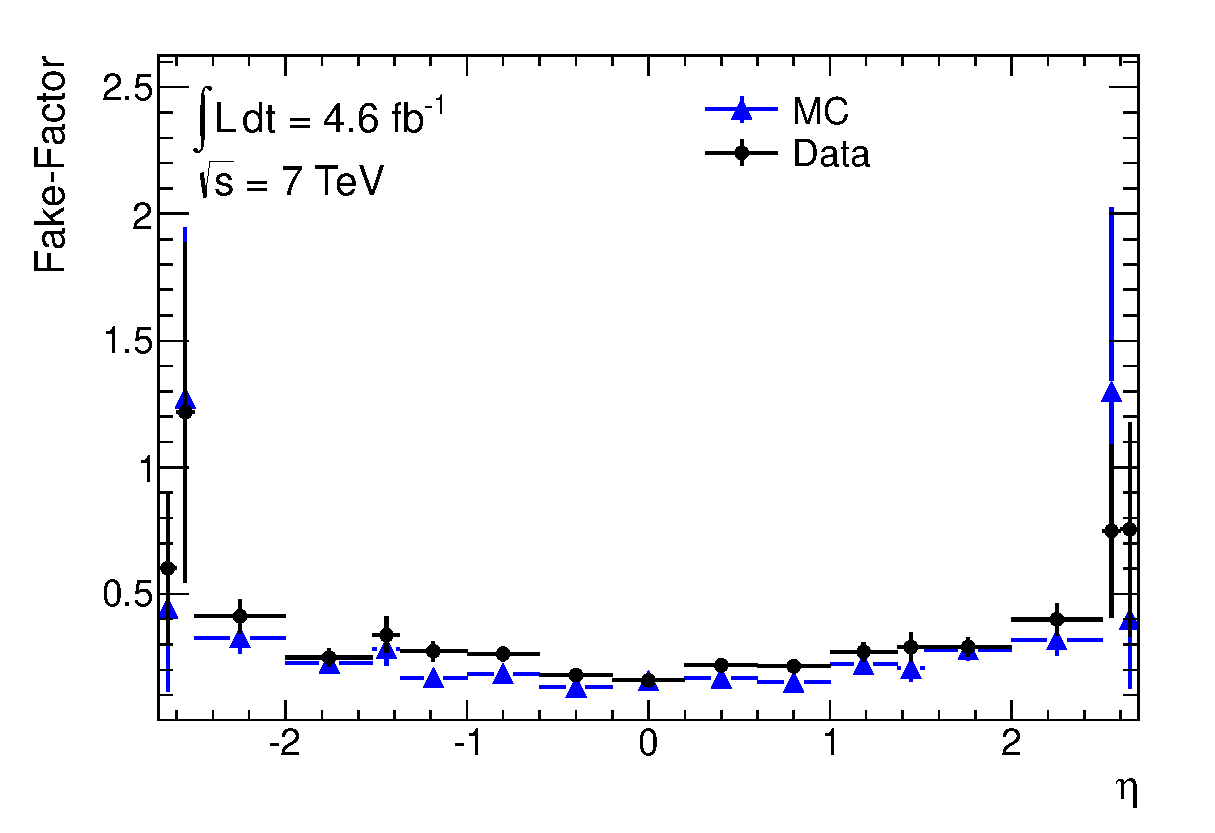
\includegraphics[width=0.47\textwidth]{FakeFactors/FF_AllMu_eta_J_lin}
%        }
%    \caption[Muon \FakeFactor s as a function of \pt\ and $\eta$ for 7~\tev\ data.]
%    {Muon \FakeFactor s as a function of \pt\ and $\eta$ for 7~\tev\ data. 
%    For the distributions as a function of \pt\, central, forward and calorimeter-tagged muons are shown
%    separately; for the $\eta$ distributions the \ffactor\ all electrons are
%    shown in the same plot.The black points show the \ffactor\ measured in
%    data; the blue triangles show the value estimated by \mc.}
%\label{fig:ff-mu-seven} 
%\end{figure}
%
%\begin{figure}[h]
%\centering
%\vspace{-8mm}
%	\subfigure[Central Muons]{
%            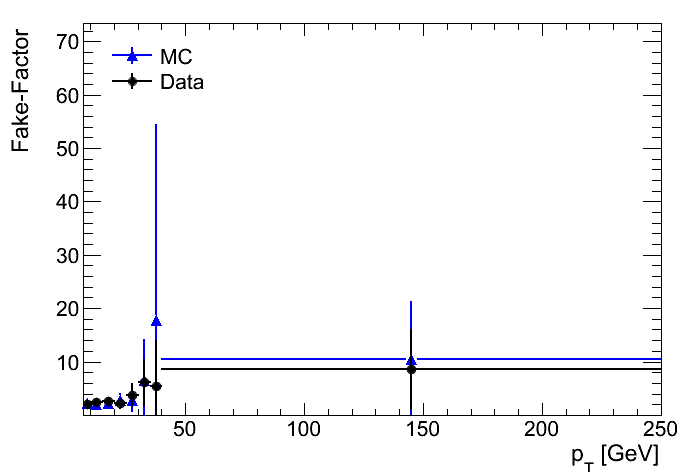
\includegraphics[width=0.47\textwidth]{FakeFactors/FF_CentralMu_pt_B_lin}
%        }
%	\subfigure[Forward Muons]{
%            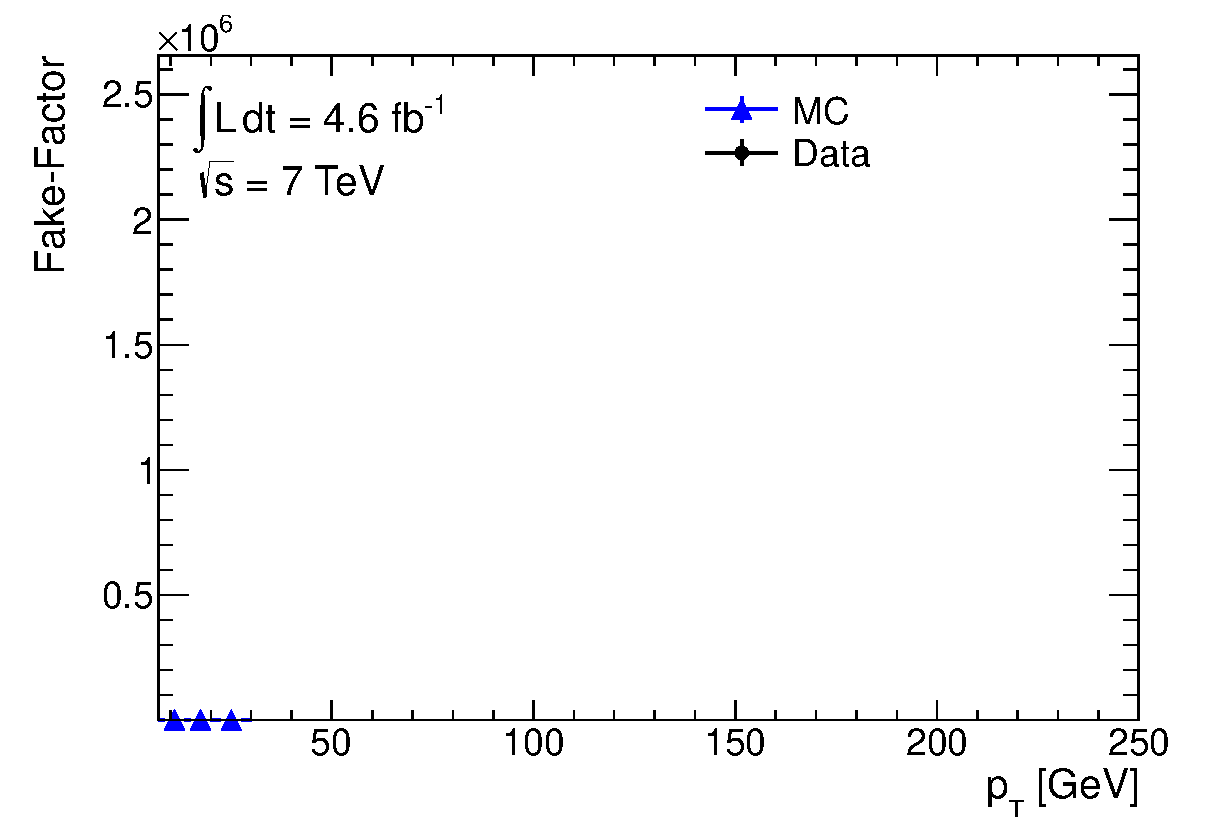
\includegraphics[width=0.47\textwidth]{FakeFactors/FF_ForwardMu_pt_B_lin}
%        }
%	\subfigure[Calorimeter-Tagged Muons]{
%            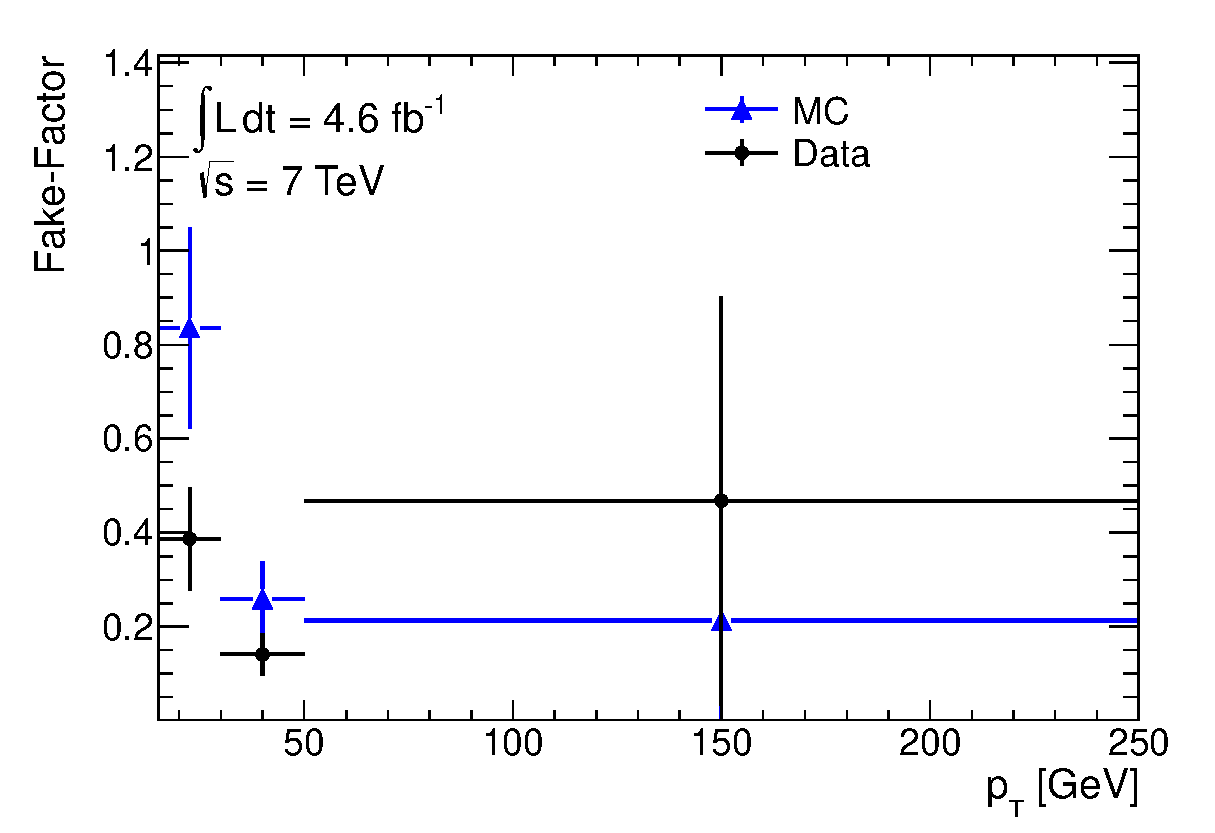
\includegraphics[width=0.47\textwidth]{FakeFactors/FF_CaloMu_pt_B_lin}
%        }
%	\subfigure[All Muons]{
%            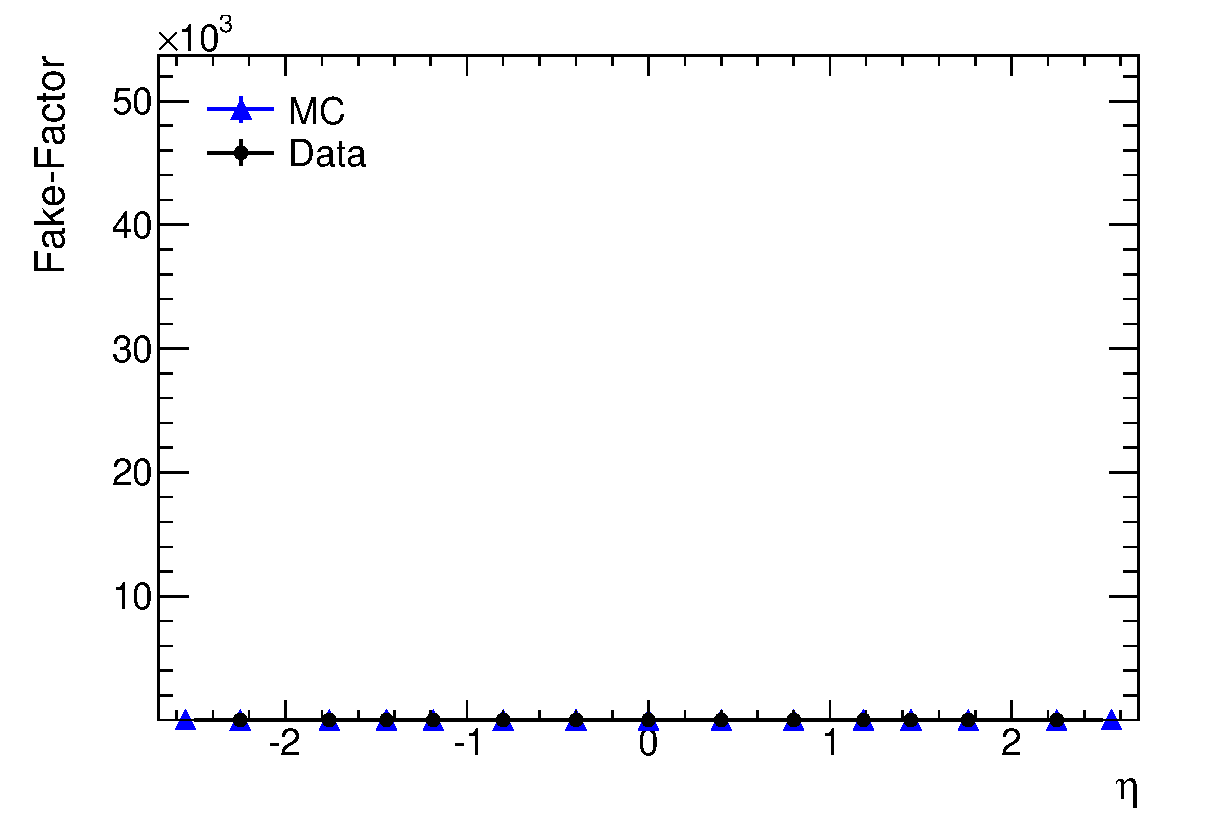
\includegraphics[width=0.47\textwidth]{FakeFactors/FF_AllMu_eta_B_lin}
%        }
%    \caption[Muon \FakeFactor s as a function of \pt\ and $\eta$ for 7~\tev\ data.]
%    {Muon \FakeFactor s as a function of \pt\ and $\eta$ for 7~\tev\ data. 
%    For the distributions as a function of \pt\, central, forward and calorimeter-tagged muons are shown
%    separately; for the $\eta$ distributions the \ffactor\ all electrons are
%    shown in the same plot.The black points show the \ffactor\ measured in
%    data; the blue triangles show the value estimated by \mc.}
%\label{fig:ff-mu-seven} 
%\end{figure}

\subsection{Results}
\subsection{Statistical and Systematic Uncertainties}
